\documentclass[11pt]{book}

\usepackage{amsfonts, amsmath, amssymb}
\usepackage{times}
\usepackage{multicol}
\usepackage[colorlinks=true, linkcolor=blue, citecolor=red, urlcolor=blue]{hyperref}
\usepackage{biblatex}
\usepackage{float}
\addbibresource{main.bib}
\usepackage{etoolbox}
\patchcmd{\chapter}{\cleardoublepage}{\clearpage}{}{}

%\usepackage[backref=page,pagebackref=true,linkcolor = blue,citecolor = red]{hyperref}
%\usepackage[backref=page]{backref}


\usepackage{graphicx}
\DeclareGraphicsExtensions{.pdf,.png,.jpg}


\setlength{\oddsidemargin}{1.5cm}
\setlength{\evensidemargin}{0cm}
\setlength{\topmargin}{1mm}
\setlength{\headheight}{1.36cm}
\setlength{\headsep}{1.00cm}
%\setlength{\textheight}{20.84cm}
\setlength{\textheight}{19cm}
\setlength{\textwidth}{14.5cm}
\setlength{\marginparsep}{1mm}
\setlength{\marginparwidth}{3cm}
\setlength{\footskip}{2.36cm}


\begin{document}
	\pagestyle{empty}

	\begin{center}

		\vspace{1cm}

%%% Type the thesis title below%%%%%%%%%%%%%%%%
		{\Huge Predictive Container Dwell Time Modeling for Optimized Port Yard Placement: A Machine Learning Approach}

		\vspace{15mm}

		
\includegraphics[width=2cm]{images/logo}

		\vspace{45mm}

%%%%%Type Your Name Below%%%%%%%%%%%%
		{\Large       Fabio Andrés García Sánchez}

		\vspace{1ex}

		School of Computer Science

		The University of Auckland

		\vspace{5ex}

		%%%%%Typing Your Supervisors Name Below%%%%%%%%%%%%
		Supervisor: Kaiqi Zhao

		\vspace{30mm}

		A dissertation submitted in partial fulfillment of the requirements for the degree of Master of
		Data Science, The University of Auckland, 2024.

	\end{center}


%: --------------------------------------------------------------
%:                  FRONT MATTER:  abstract,..
% --------------------------------------------------------------
	\chapter*{Abstract}
	\setcounter{page}{1}
	\pagestyle{headings}
% \pagenumbering{roman}

	\addcontentsline{toc}{chapter}{Abstract}


	\begin{abstract}
		This research industry project presents a machine learning approach to predict container dwell times at the
		Ports of Auckland, aiming to optimize yard operations through data-driven decision support. The study analyzed
		over 1.5 million container movement records to develop predictive models that could effectively categorize
		container dwell times into three meaningful ranges: short-term (0-3 days), medium-term (4-11 days), and
		long-term (12+ days). Multiple machine learning algorithms were evaluated, including Random Forest, K-Nearest
		Neighbors, Logistic Regression, and Gradient Boosting. Logistic Regression was the most effective model,
		achieving F1 scores consistently above
		73\% in weekly predictions during the first quarter of 2024, with solid performance in short-term ( 86\% F1
		score) and medium-term (80\% F1 score) predictions. K-Nearest Neighbors demonstrated complementary capabilities
		as a secondary validation model. The research established that container characteristics and temporal
		patterns were significant predictors of dwell time, while environmental factors such as wind conditions
		recorded by Ports of Auckland, provided for training, showed no meaningful impact on prediction accuracy.
		Models' strong performance in short- and medium-term scenarios, represented in most operational cases,
		indicated their readiness for practical implementation. Both models struggled with long-term predictions.
		This study also proposed integrating these predictive models into a Decision Support System (DSS) to automate
		container allocation decisions to reduce unnecessary container movements and improve space utilization. The
		findings provide bases for enhancing operational efficiency in port yard management, with clear pathways for
		future development through extended data collection, granular yard-level analysis, and real-time DSS
		implementation.
	\end{abstract}

	\chapter*{Acknowledgment}

	The journey of completing this dissertation has been transformative, made possible by the extraordinary support of
	many remarkable individuals.
	\\
	\\
	I am profoundly grateful to the Port of Auckland, especially Manvi Madan and Valerie Wijaya, whose collaboration
	went far beyond professional courtesy. Their understanding during my health challenges and willingness to adapt to
	my circumstances made this research possible.
	\\
	\\
	Two exceptional mentors guided my journey. To my supervisor, Dr. Kaiqi Zhao, thank you for your intellectual
	guidance, which consistently challenged me to reach higher standards while showing patience and understanding
	when I needed it most. Susanne Cooke, our Industry Engagement Manager, you were more than just a professional guide
	– your timely advice on managing health challenges alongside research responsibilities proved invaluable. Together,
	you shaped my research and understanding of proper academic mentorship.
	\\
	\\
	In the moments when the path seemed most challenging, I found strength through the support of the university's
	student services team. Chanel Tafa from Campus Care and Emma Cooper-Williams, our Student Support Adviser, your
	compassionate guidance helped me navigate personal hurdles while keeping my academic dreams alive. You showed me
	that seeking support is not a sign of weakness but a step toward resilience.
	\\
	\\
	To my beloved wife, your decision to build a new life with me in New Zealand speaks volumes about your love and
	commitment. Your strength was outstanding, holding everything in place as we learned about becoming parents while I
	did this dissertation. Your faith in me has been my guiding light through late nights of research and moments of
	doubt. This achievement is as much yours as it is mine, and sharing this journey of academic growth while preparing
	for parenthood has made it infinitely more meaningful.
	\\
	\\
	This dissertation represents industry research and an example of human connection and support. Each person
	mentioned here has contributed to this scholarly work and my growth as a professional, a husband, and a soon-to-be
	father. For this, I am eternally grateful.

	\tableofcontents

	\chapter{Introduction}%    \chapter{}  = level 1, top level
	Imaging a place where thousands of boxes called containers flow through daily, carried by cranes or ships berth,
	orchestrating each movement to finally place them in a well-organized pile, set to be handled, rehandled,
	built, and retrieved when the time comes, to leave the port. For this logistical marvel, there is a critical
	challenge in this process: predicting, with precision, how long each box will stay to ensure they are moved only
	when necessary for their onward journey rather than to accommodate other cargo. This predictive capability can
	streamline port operations to reduce unnecessary movements while optimizing space utilization. This puzzle of
	time for improving movement and placements is the main point of this dissertation's inquiry.
	\\
	\\
	In today's fast-paced world of global trade, container ports are like the beating hearts of our supply chains.
	However, here is the thing: these ports face a constant puzzle – how to manage their limited space most
	efficiently. This is not about squeezing in as many containers as possible but knowing which ones will leave
	soon or stick around for a while.
	\\
	\\
	This research project was born from a collaboration with the Port of Auckland to find a way to use the data to
	optimize yard operations somehow. Following that mandate, using statistics, historical data, and the container’s
	movements and features, this project proposed building predictive models to predict dwell times
	\cite{merckx2005issue}
	, implementing machine learning techniques that can be involved inside the decision support system DSS (
	Figure~\ref{fig:dds_architecture}
	) to help day-to-day operations by making decisions based on predicting plausible days of container stays.
	\\
	\\
	That is where this research comes in to develop a machine learning model for doing something interesting: predict
	how long containers will stay in the port. However, why does this matter? What is the dissertation's primary goal?
	Predicting how long containers would hang around in the port (the trained predictive models) for being used as an
	input of a decision support system to optimize the yard operations.
	\\
	\\
	Think of it this way: if port managers know Container A will be picked up in two days while Container B will hang
	around for a week, they can make smarter decisions about where to put them (stacking strategies). It is similar
	to a high-stakes Tetris game but with costly real-world consequences.
	\\
	\\
	The proposed models are about more than just making educated guesses but are built for helping to solve challenges
	related to port operations:

	\begin{enumerate}

		\item Container Stacking Problem (CSP) \cite{galle2018stochastic}: The dwell time prediction helps to stack
		containers more effectively by reducing unnecessary movements. Those containers with shorter stays are
		placed on top, reducing relocations in future retrieval while improving operational efficiency.

		\item
		Storage Space Allocation Problem (SSAP) \cite{da2019reactive}: By using dwell time predictions, the
		containers could be assigned to the yard based on how long they will stay, trying to leave short-term
		containers in easily accessible areas.

		\item
		Container Retrieval Problem (CRP) \cite{da2019reactive}
		: Predicting dwell times helps organize containers efficiently for retrieval.
		Containers organized in a sequence leads to faster and smoother loading operations.

		\item Container Relocation Problem (CRP/BRP) \cite{lin2015container}: Dwell time predictions reduce
		unnecessary relocations by placing containers strategically with similar exit times together or in a
		strategic order, minimizing disruptions while lowering the costs of moving containers multiple times.

	\end{enumerate}
	\\
	\\
	Here is the exciting part: All placement decisions should be made based on some rules considering the container's
	dwell time. This research aims to provide models for that by providing data-driven insights for reducing
	unnecessary container shuffling, saving time, cutting costs, and even reducing the environmental impact of port
	operations.
	\\
	\\
	This dissertation will describe how these predictive models were built, the data used, and the machine learning
	techniques employed. It also shows how well it performs. This is about crafting a clever algorithm and
	improving how
	ports operate. This research aims to set additional tools to contribute to intelligent, efficient container
	handling by using the data and integrating an additional approach from data science theory to port operations.


	\section{System Architecture and Research Focus}

		Figure~\ref{fig:dds_architecture}
		illustrates a comprehensive two-tier system architecture that combines a Trained Predictive Model
		with a Decision Support System (DSS). This research focuses specifically on developing and optimizing
		the Trained Predictive Model component, which serves as the foundation for future yard optimization
		applications.
		\\
		\\
		The Trained Predictive Model component is the core of this research. It integrates two fundamental data
		sources: Container Features, which include physical and operational characteristics from containers, and Time
		Features, which capture temporal patterns and timing-related data. Multiple classifiers process them to
		generate predicted dwell time ranges.
		\\
		\\
		While the development of a complete DSS lies beyond the scope of this research, the architecture demonstrates
		how the predictive model could be integrated into a broader operational framework. The DSS reference is
		structured into two operational layers: Weekly Planning and Yard Operation. On the one hand, the Weekly
		Planning layer processes yard container data to generate predictions for current containers inside the yard,
		supporting medium-term operational planning. On the other hand, the Yard Operation layer handles real-time
		decisions by processing individual container features to predict dwell ranges for incoming containers,
		informing immediate stacking strategies and container allocation decisions. Both use the dwell times from
		predictions.
		\\
		\\
		This dissertation focuses on predicting container dwell times across three ranges: short-term (0-3 days),
		medium-term (4-11 days), and long-term (12+ days), serving a practical purpose in yard operations: transforming
		raw predictions into actionable insights. By integrating ranges of dwell times into a Decision Support System
		(DSS), predictions could improve operations, enabling more informed container placement decisions that minimize
		unnecessary container movements and ultimately enhance the port's overall operational efficiency.

		\begin{figure}[ht]
			\centering
			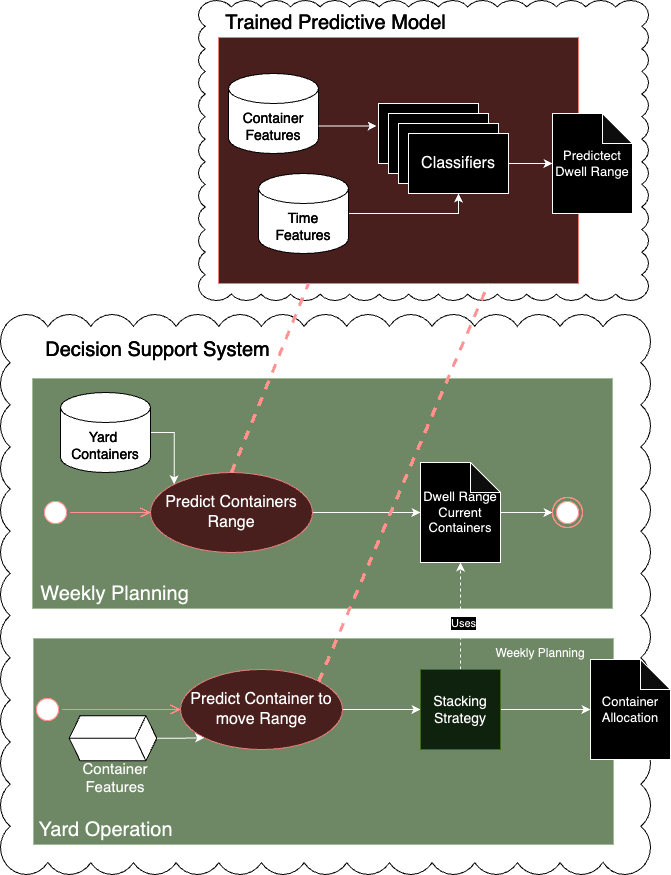
\includegraphics[width=1\textwidth]{images/DSS}
			\caption{DSS architecture using machine learning models}
			\label{fig:dds_architecture}
		\end{figure}


	\chapter{Literature Review / Related Works}%    \chapter{}  = level 1, top level
	Container stacking and decision support systems (DSS) have evolved significantly in port operations management.
	\\
	\\
	While numerous studies have addressed container stacking problems
	\cite{gharehgozli2014decision, ries2014fuzzy, bazzazi2009genetic, guven2019modelling, guerra2018heuristic,
		nishimura2009container, sharma2014genetic, park2011dynamic, goerigk2016robust}, developing comprehensive DSS
	solutions has been relatively limited. Notable exceptions include the work of Murty et al.
	\cite{murty2005decision}, Liu et al. \cite{liu2010decision}, and Legato and Mazza \cite{legato2018decision},
	though these studies did not integrate predictive analytics or consider dwell times in their optimization models.
	\\
	\\
	Even though dwell time performance is an important indicator, affected by multiple factor (Table~
	\ref{tab:dwell_time_factors}
	), a gap exists in the literature regarding container dwell time prediction to solve optimization yard
	problems. Only some studies address this challenge; Moini et al. \cite{moini2012estimating}
	analyzed U.S. ports, identifying crucial features such as port type, geographical location, and container traffic
	patterns. Based on this foundation, Kourounioti et al. \cite{kourounioti2016development}
	employed regression models and neural networks to predict dwell time.
	\\
	\\
	The hierarchical approach to decision-making has emerged as a common framework in container terminal
	operations.
	As documented by several researchers \cite{zhang2003storage, chen2012storage, park2011dynamic}, this two-stage
	process first considers block assignment at an aggregated level, followed by real-time decisions about specific
	container locations. Some insights about storage yard operations are provided by Carlo et al.
	\cite{carlo2014storage}.
	\\
	\\
	Historical perspectives reveal the evolution of DSS applications for container handling. Starting with the
	early contribution from Van Hee and Wijbrands \cite{van1988decision}, the field has expanded to cover many
	operational aspects.
	Recent studies have addressed specific challenges such as real-time transportation planning
	\cite{bandeira2009dss, van2016real, shen1995dss}, crane scheduling, berth allocation
	\cite{wang2007stochastic}, and the integrated berth allocation and quay crane assignment Problem (BACAP) problem
	\cite{ursavas2014decision}.
	\\
	\\
	The effectiveness of category-based stacking policies in reducing rehandles has been well-documented. As a
	reference, Dekker et al. \cite{dekker2007advanced} demonstrated the benefits of category-based stacking. On the
	other hand, Borgman et al. \cite{borgman2010online} have highlighted the importance of departure time-based
	classification. Historical data can reduce operational costs, improving service levels for port users by
	leveraging and designing more effective stacking rules.
	\\
	\\
	This research builds upon a study by Gaete et al. \cite{gaete2018novel}, which explored dwell time prediction using
	multi-class classification. Also, follows some of the ideas for a DSS architecture proposed by Maldonado et al.
	\cite{maldonado2019analytics} which uses machine learning models for decision-making in port operations across a
	decision support system.
	\\
	\\
	The current approach introduces a methodology for dwell time prediction by classifiers adjusted to The Ports of
	Auckland's operational context. It explains how these predictions could be integrated into DSS architecture that
	could be implemented in real-world port operations to optimize the yard finally.

	\begin{table}[ht]
		\centering
		\begin{tabular}{|p{0.45\textwidth}|c|c|}
			\toprule
			\hline
			\textbf{Factor} & \textbf{References}
			& \textbf{Type} \\
			\hline
			\midrule
			Vessel sailing schedule frequency & \cite{merckx2005issue, moini2012estimating}
			& Unique value
			\\
			\hline
			Container specifications\textsuperscript{*} & \cite{merckx2005issue, moini2012estimating}
			& Nominal
			\\
			\hline
			Hinterland connections & \cite{merckx2005issue, moini2012estimating}
			& Unique value \\
			\hline
			Port governance structure & \cite{merckx2005issue, moini2012estimating}
			& Unique value \\
			\hline
			Terminal location \& logistics & \cite{merckx2005issue, moini2012estimating}
			& Unique value
			\\
			\hline
			Terminal operations schedule &
			\cite{merckx2005issue, moini2012estimating, rodrigue2009terminalization}
			& Unique value
			\\
			\hline
			Shippers and consignees & \cite{moini2012estimating, rodrigue2009terminalization}
			& Nominal
			\\
			\hline
			Regulatory procedures & \cite{moini2012estimating}
			& Unique value \\
			\hline
			Transport corridors & \cite{moini2012estimating}
			& Nominal \\
			\hline
			Maritime shipping details\textsuperscript{†} & \cite{moini2012estimating}
			& Nominal \\
			\hline
			Container flow balance & \cite{moini2012estimating}
			& Nominal \\
			\hline
			\bottomrule
			\multicolumn{3}{l}
			{\footnotesize \textsuperscript{*}Including type (empty/full, dry/reefer), size (20/40 TEUs), contents}
			\\
			\multicolumn{3}{l}{\footnotesize \textsuperscript{†}Ocean carriers and empty container demurrage time}
			\\
		\end{tabular}
		\caption{Factors Influencing Container Dwell Time \cite{gaete2018novel}}
		\label{tab:dwell_time_factors}
	\end{table}

	\chapter{Dataset}%    \chapter{}  = level 1, top level


	\section{Introduction to container dataset}
		The dataset has records regarding container terminal operations. More over 1.5 million observations and 35
		variables provide a detailed details container movements, including imports, exports, and container features.


	\section{Data Features Overview}

		The dataset encompasses a comprehensive set of features that characterize container operations at the port.
		These features can be categorized into five main groups. As shown in Table \ref{tab:container_chars}
		, categorical features include container physical characteristics such as nominal length (20, 40,
		45, or 10 feet) and location types. The operational categories, detailed in Table \ref{tab:category_features}
		, include import (IMPRT), export (EXPRT), storage (STRGE), transshipment (TRSHP), and through cargo (
		THRGH). Table \ref{tab:move_kind}
		outlines the movement types captured through various categories like delivery (DLVR), loading (LOAD),
		yard moves (YARD), and others, while freight types are classified in Table \ref{tab:freight_kind}
		as either empty (MTY) or full container load (FCL).

		\begin{table}[H]
			\centering
			\begin{tabular}{p{0.2\textwidth}p{0.7\textwidth}}
				\hline
				\textbf{Column Name} & \textbf{Description}
				\\
				\hline
				nominal\_length & Container size that could be 20, 40, 45, and 10
				\\
				\hline
				arrive\_pos\_loctype & Type of location arrival
				\\
				\hline
				last\_pos\_loctype & Last position's type where the container was fetched from, related to fm\_pos
				\_locid \\
				\hline
			\end{tabular}
			\caption{Container Characteristics Features}
			\label{tab:container_chars}
		\end{table}

		\begin{table}[H]
			\centering
			\begin{tabular}{p{0.15\textwidth}p{0.7\textwidth}}
				\hline
				\textbf{Category} & \textbf{Description}                                                  \\
				\hline
				IMPRT                 & Import                                                                \\
				\hline
				EXPRT                 & Export                                                                \\
				\hline
				STRGE                 & Storage                                                               \\
				\hline
				TRSHP                 & When a box comes off a vessel and goes on another vessel              \\
				\hline
				THRGH                 & When a box leaves on the same vessel it came on, it just went through \\
				\hline
			\end{tabular}
			\caption{Container Category Features}
			\label{tab:category_features}
		\end{table}

		\begin{table}[H]
			\centering
			\begin{tabular}{p{0.15\textwidth}p{0.7\textwidth}}
				\hline
				\textbf{Category} & \textbf{Description} \\
				\hline
				DLVR                  & Delivery             \\
				\hline
				LOAD                  & Load                 \\
				\hline
				YARD                  & Yard Move            \\
				\hline
				SHFT                  & Yard Shift           \\
				\hline
				RECV                  & Receival             \\
				\hline
				RLOD                  & Rail load            \\
				\hline
				OTHR                  & Other                \\
				\hline
				RDSC                  & Rail Discharge       \\
				\hline
				DSCH                  & Discharge            \\
				\hline
				SHOB                  & Shift O.B            \\
				\hline
			\end{tabular}
			\caption{Move Kind Features}
			\label{tab:move_kind}
		\end{table}

		\begin{table}[H]
			\centering
			\begin{tabular}{p{0.15\textwidth}p{0.7\textwidth}}
				\hline
				\textbf{Category} & \textbf{Description} \\
				\hline
				MTY                   & Empty                \\
				\hline
				FCL                   & Full Container Load  \\
				\hline
			\end{tabular}
			\caption{Freight Kind Features}
			\label{tab:freight_kind}
		\end{table}

		Binary features, presented in Table \ref{tab:binary_features}
		, track specific operational requirements such as power needs for temperature-sensitive cargo and twin
		operation capabilities (fetch, carry, and put).

		\begin{table}[H]
			\centering
			\begin{tabular}{p{0.2\textwidth}p{0.7\textwidth}}
				\hline
				\textbf{Column Name} & \textbf{Description}
				\\
				\hline
				requires\_
				power & Container designed to be transported as temperature sensitive cargo with precisely
				controlled temperatures \\
				\hline
				twin\_fetch & Pairs of containers that were able be twin fetched
				\\
				\hline
				twin\_carry & Pairs of containers that can able be twin carried
				\\
				\hline
				twin\_put & Time when the whole chain of events related to a container\_visit\_
				gkey is completed \\
				\hline
			\end{tabular}
			\caption{Binary Features}
			\label{tab:binary_features}
		\end{table}

		Temporal information is captured through datetime features, listed in Table \ref{tab:datetime_features}
		, that record crucial timestamps including port arrival (time\_in), departure (time\_out), and various
		handling operations (t\_put, t\_dispatch, t\_fetch, t\_discharge).
		\begin{table}[H]
			\centering
			\begin{tabular}{p{0.2\textwidth}p{0.7\textwidth}}
				\hline
				\textbf{Column Name} & \textbf{Description}
				\\
				\hline
				t\_put & Time completed
				\\
				\hline
				t\_dispatch & Time when a container is dispatched somewhere like on a vessel or truck
				\\
				\hline
				t\_carry\_dispatch & Requires verification
				\\
				\hline
				t\_fetch & Datetime when the container was fetched
				\\
				\hline
				t\_discharge & Datetime when container is left in position after being fetched
				\\
				\hline
				time\_
				in & Datetime of port arrival (for transships: can indicate category change from
				storage
				to export) \\
				\hline
				time\_out & Time when the container leaves the port
				\\
				\hline
			\end{tabular}
			\caption{Datetime Features}
			\label{tab:datetime_features}
		\end{table}

		Table \ref{tab:numerical_features}
		outlines numerical features that provide quantitative data about container handling, including rehandle
		counts, weight measurements (goods\_an\d_ctr\_wt\_kg), and movement distances (dist\_start, dist\_carry).
		\begin{table}[H]
			\centering
			\begin{tabular}{p{0.2\textwidth}p{0.7\textwidth}}
				\hline
				\textbf{Column Name} & \textbf{Description}
				\\
				\hline
				rehandle\_count & Number of times a container was rehandled
				\\
				\hline
				goods\_and\_ctr\_wt\_kg & Total weight of goods and container
				\\
				\hline
				dist\_start & Distance where container started to be moved
				\\
				\hline
				dist\_
				carry & Distance container was carried during move (correlated to starting distance) \\
				\hline
			\end{tabular}
			\caption{Numerical Features}
			\label{tab:numerical_features}
		\end{table}

		Finally, identifier features, detailed in Table \ref{tab:identifier_features}
		, maintain traceability through unique keys for moves (mve\_gkey), locations (fm\_pos\_locid,
		to\_pos\_locid)
		, containers (inv\_unit\_id), and operators (bizunit\_id).

		\begin{table}[H]
			\centering
			\begin{tabular}{p{0.2\textwidth}p{0.7\textwidth}}
				\hline
				\textbf{Column Name} & \textbf{Description}                                    \\
				\hline
				mve\_gkey                & Unique identifier for each move                         \\
				\hline
				fm\_pos\_locid           & FROM Position location id associated with fm\_pos\_name \\
				\hline
				fm\_pos\_name            & Name of the location associated with fm\_pos\_locid     \\
				\hline
				to\_pos\_locid           & TO Position location associated with to\_pos\_name      \\
				\hline
				to\_pos\_name            & Name of the location associated with to\_pos\_locid     \\
				\hline
				inv\_unit\_id            & Container ID (persistent across port visits)            \\
				\hline
				bizunit\_id              & Line operator's ID                                      \\
				\hline
			\end{tabular}
			\caption{Identifier Features}
			\label{tab:identifier_features}
		\end{table}


	\section{Data Preprocessing}

		\subsection{Data Augmentation}

			From existing features (table~\ref{tab:datetime_features}
			),new ones like the month, day, week of the month, day of the week, and even the time each container
			arrived were created based on the dates. Also, the number of days for each container, related to dwell
			time, was calculated using the dates in and out, creating the feature: "Days in the port category," a range
			of days.

		\subsection{Data Cleaning}

			The dataset was almost complete for the approach. However, some formats had to be set properly, from
			strings to dates. It had some columns with flags (like requires\_
			power) that had missing values. For these, an imputation with 0 was done.

		\subsection{Data Reduction}
			Our final dataset was reduced into 480,625 rows, each representing a unique container stay with ten chosen
			features split into two main chunks:

			\begin{itemize}
				\item 376,557 rows from 2023 for training and initial testing
				\item 104,068 rows from 2024 kept separate as our unseen data for final testing
			\end{itemize}
			The year 2024 was set up to test the model's performance on truly new data – the ultimate test of its
			predictive power.
			\\
			\\
			Many columns containing IDs, session user information, dates, and flags outside the goal of predicting
			dwell time were removed.
			\\
			\\
			After selecting the most important columns, the ones included were container's physical characteristics (
			nominal length), operational requirements (requires power status), and cargo attributes (freight kind and
			category). The temporal aspects were captured through multiple granularities: time of day (hour), day of
			week, month, business day status, week of year, and week of month.


	\section{Data analysis}

		\subsection{Initial Exploratory Approach}
			The research began with an open-ended mandate from the Ports of Auckland to analyze their operational data
			to look for potential yard optimization insights. Rather than starting with a predefined hypothesis, this
			project follows an exploratory data science approach to discover patterns and opportunities from the
			provided data. The database structure was initially understood by examining column types and their values.
			Each finding pattern was evaluated with the stakeholders from Ports of Auckland.

		\subsection{Tool Selection: R}
			R was selected for the initial data exploration because of its robust statistical analysis and
			visualization tools. Packages such as ggplot2 enabled detailed visualizations, and data packages allowed
			efficient handling of large datasets. RStudio\’s interactive environment provided quick visual feedback,
			making it easy to try different approaches rapidly. R\’s built-in statistical functions and intuitive data
			manipulation also made it ideal for exploratory work in this phase.
			\\
			\\
			R provided several clear benefits compared to Python, which was also a potential choice for data
			exploration. Its syntax allows data manipulation to be faster and easier. Also, its high-quality default
			plotting aesthetics minimized the need for extensive customization, allowing advanced customization when
			needed.
			\\
			\\
			R\’s built-in solid statistical analysis tools delivered immediate insights without extra library
			installations, and its efficient memory management was essential for effectively handling the sizeable
			operational dataset.
			\\
			\\
			This data exploration is provided in \cite{githubrepo}.

		\subsection{Iterative Development Process}
			The methodology for this project follows an iterative approach that involves an in-depth data exploration
			using R, which exposed potential optimization areas. The insights generated in this phase were part of
			follow-up discussions with Ports of Auckland stakeholders to ensure they were aligned with real operational
			needs.

		\subsection{Data Exploration}

			\begin{figure}[ht]
				\centering
				\begin{minipage}{0.5\textwidth}
					\centering
					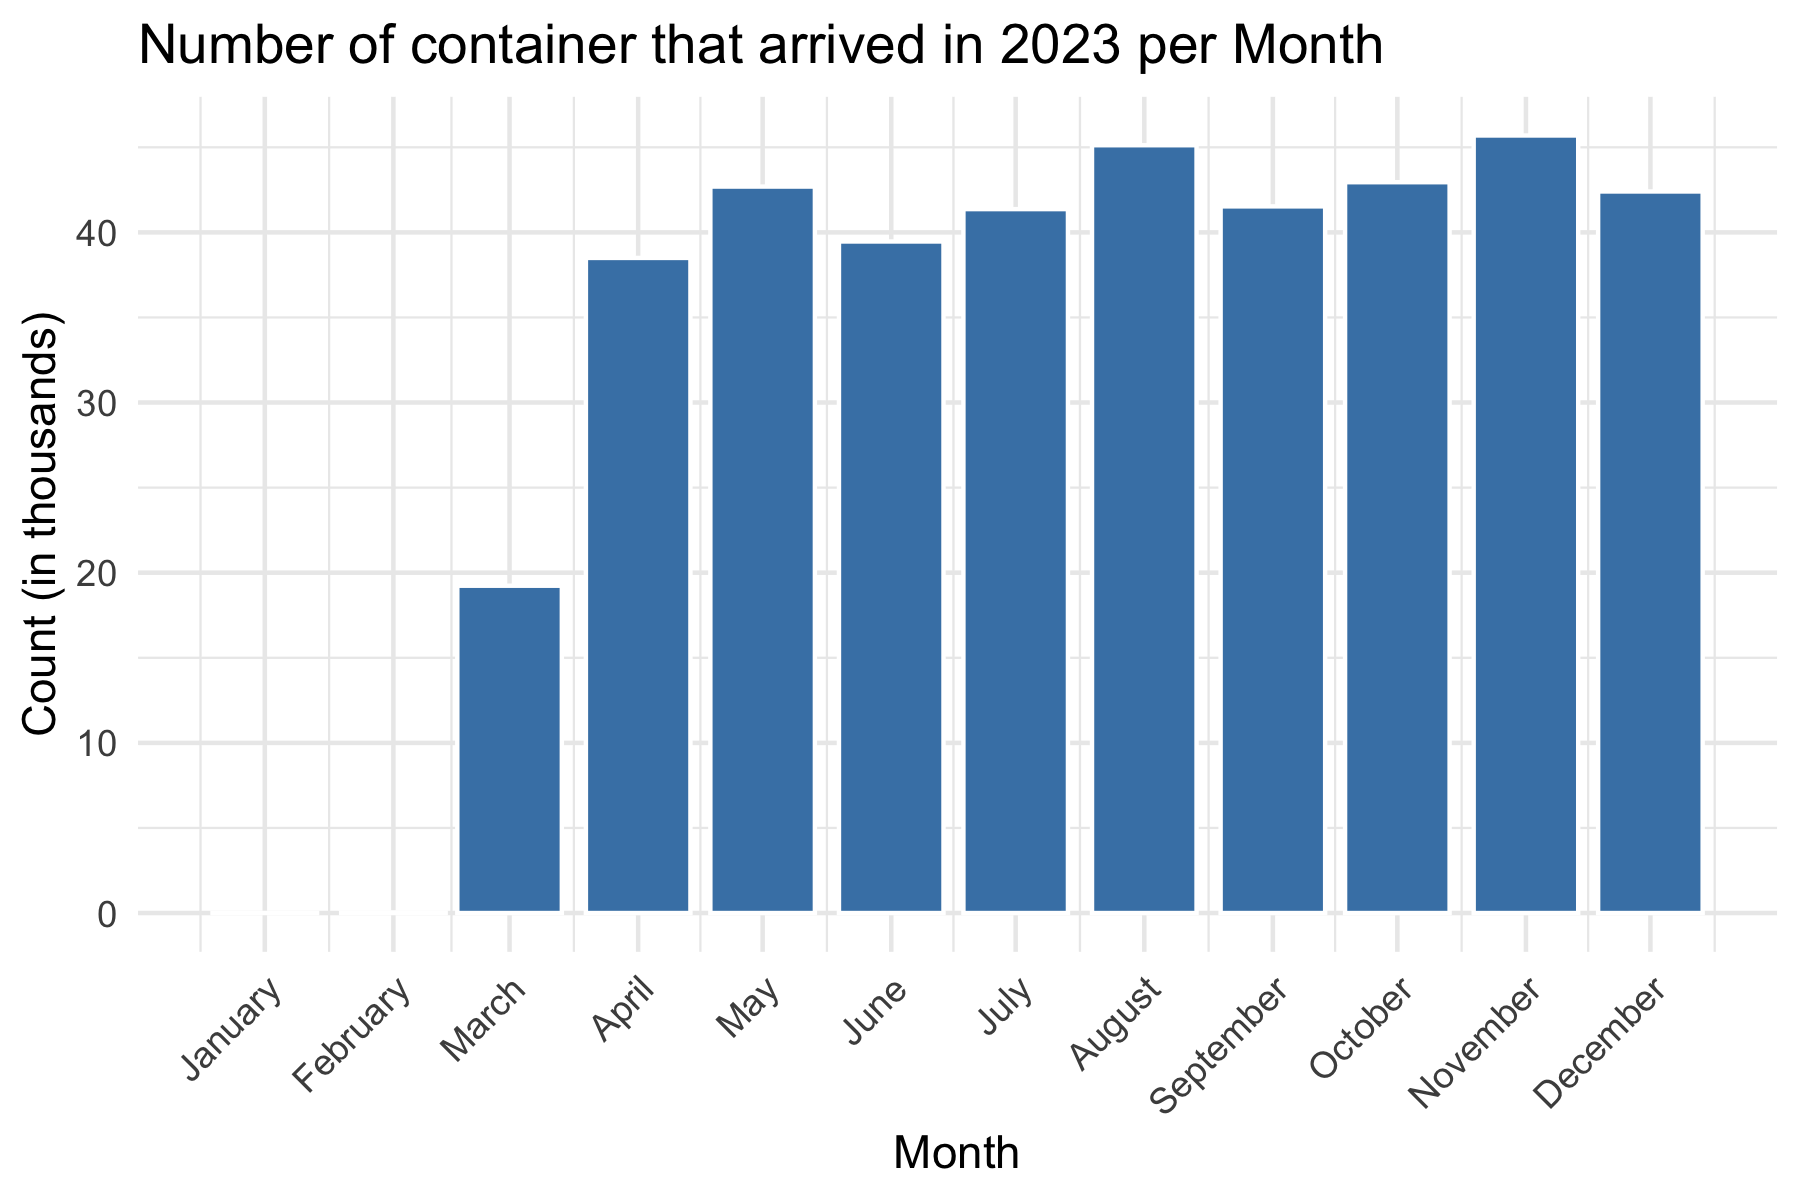
\includegraphics[width=\textwidth]{images/du_zero_one}
					\caption{Container arrivals at a port 2023}
					\label{fig:du_containers_arrivals_2023}
				\end{minipage}%
				\hfill
				\begin{minipage}{0.5\textwidth}
					\centering
					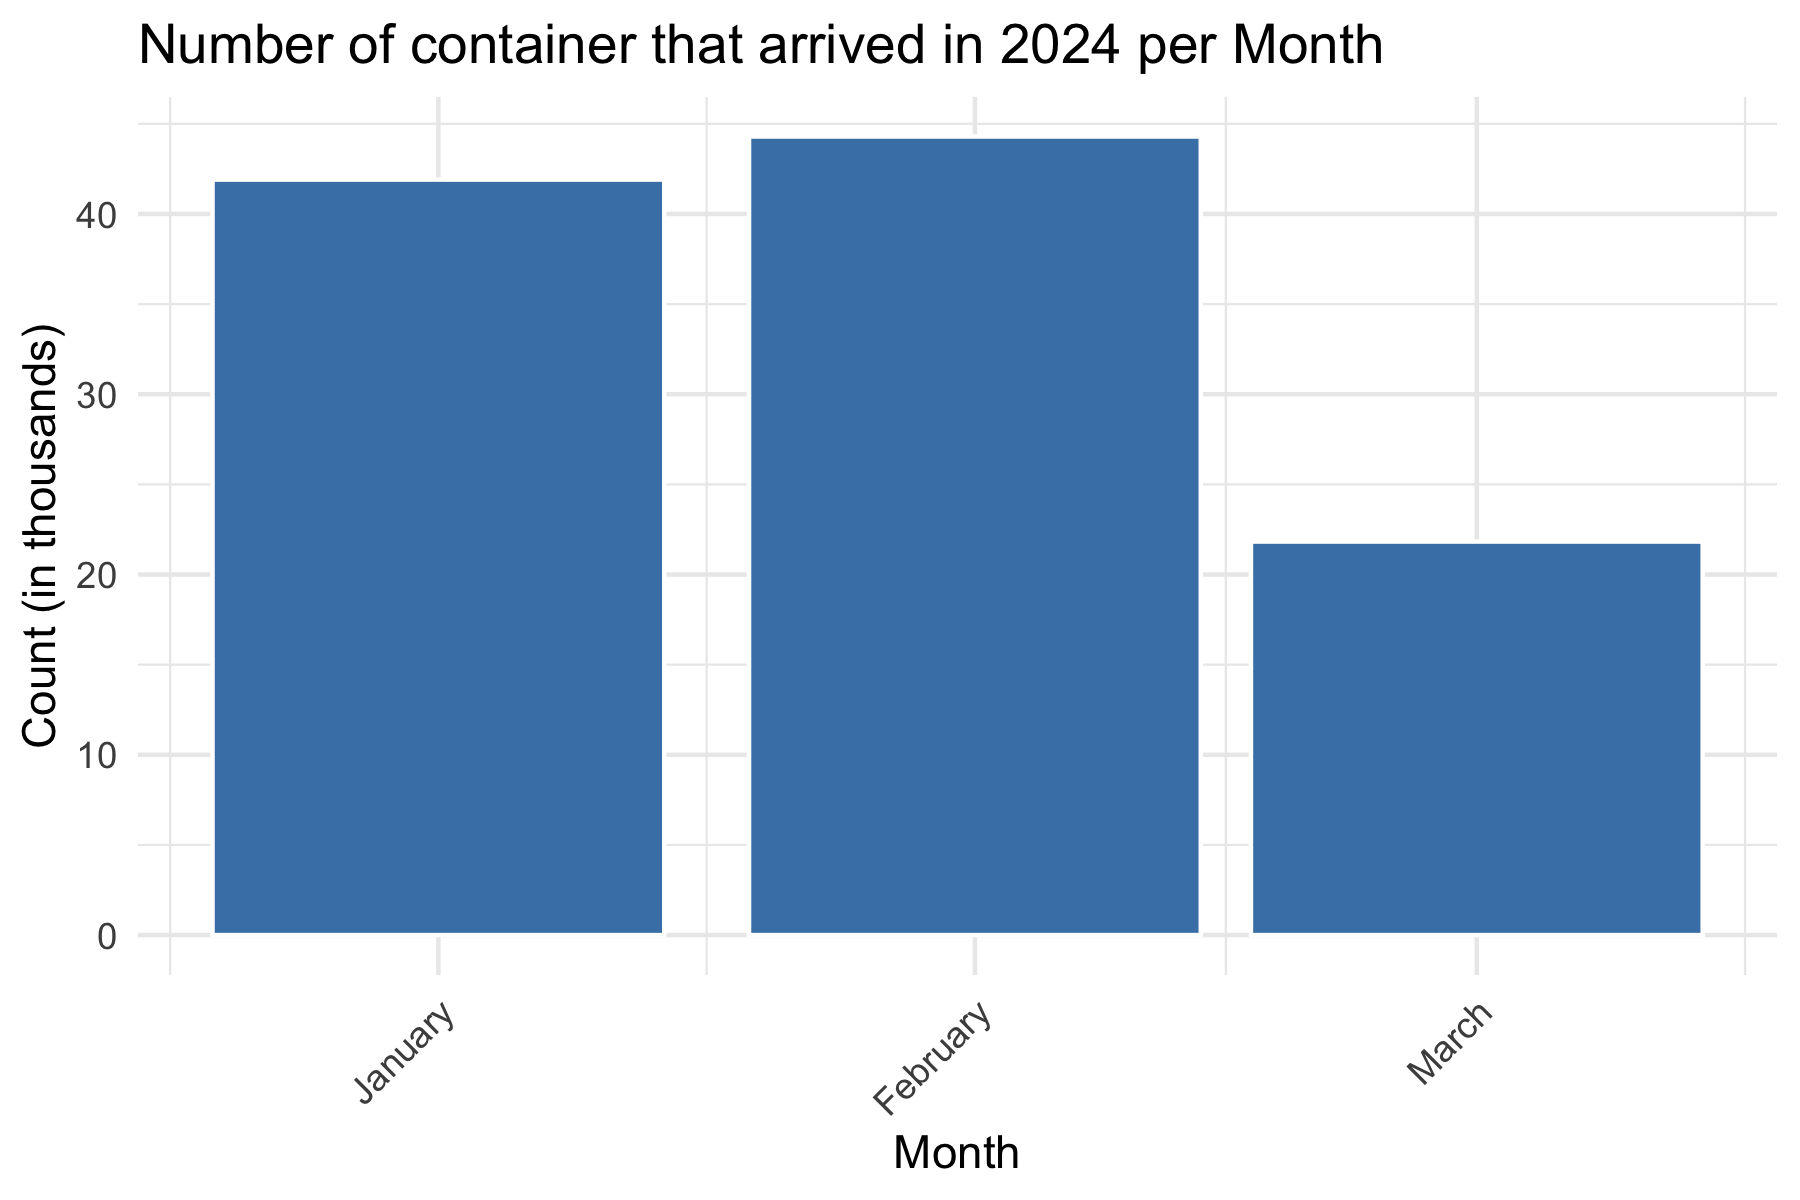
\includegraphics[width=\textwidth]{images/du_zero_two}
					\caption{Container arrivals at a port 2024}
					\label{fig:du_containers_arrivals_2024}
				\end{minipage}
			\end{figure}

			Figure~\ref{fig:du_containers_arrivals_2023}
			illustrates the monthly container arrivals at a port, measured in thousands of units, spanning
			from January 2023 to March 2024, with the 2024 cycle needing to be completed as it only covers the
			first quarter. For the year 2023, there is no available data for January and February. It includes
			half the month of March with approximately 19,000 containers.
			\\
			\\
			For April, the amount of containers reached about 38,000 containers. Throughout the remainder of
			2023, the port maintained relatively stable activity levels from May through December, with monthly
			container arrivals fluctuating between 39,000 and 45,000 units. A peak activity was observed in September,
			with approximately 45,000 containers concluding in December, with approximately 42,000 container arrivals.
			\\
			\\
			The available data for 2024 (Figure~\ref{fig:du_containers_arrivals_2024}), which only spans the first
			quarter, shows that January began with approximately 42,000 container arrivals, followed by a slight
			increase to about 45,000 containers in February. However, March contains just the first two weeks of the
			month with approximately 22,000 containers.
			\\
			\\
			\begin{figure}[ht]
				\centering
				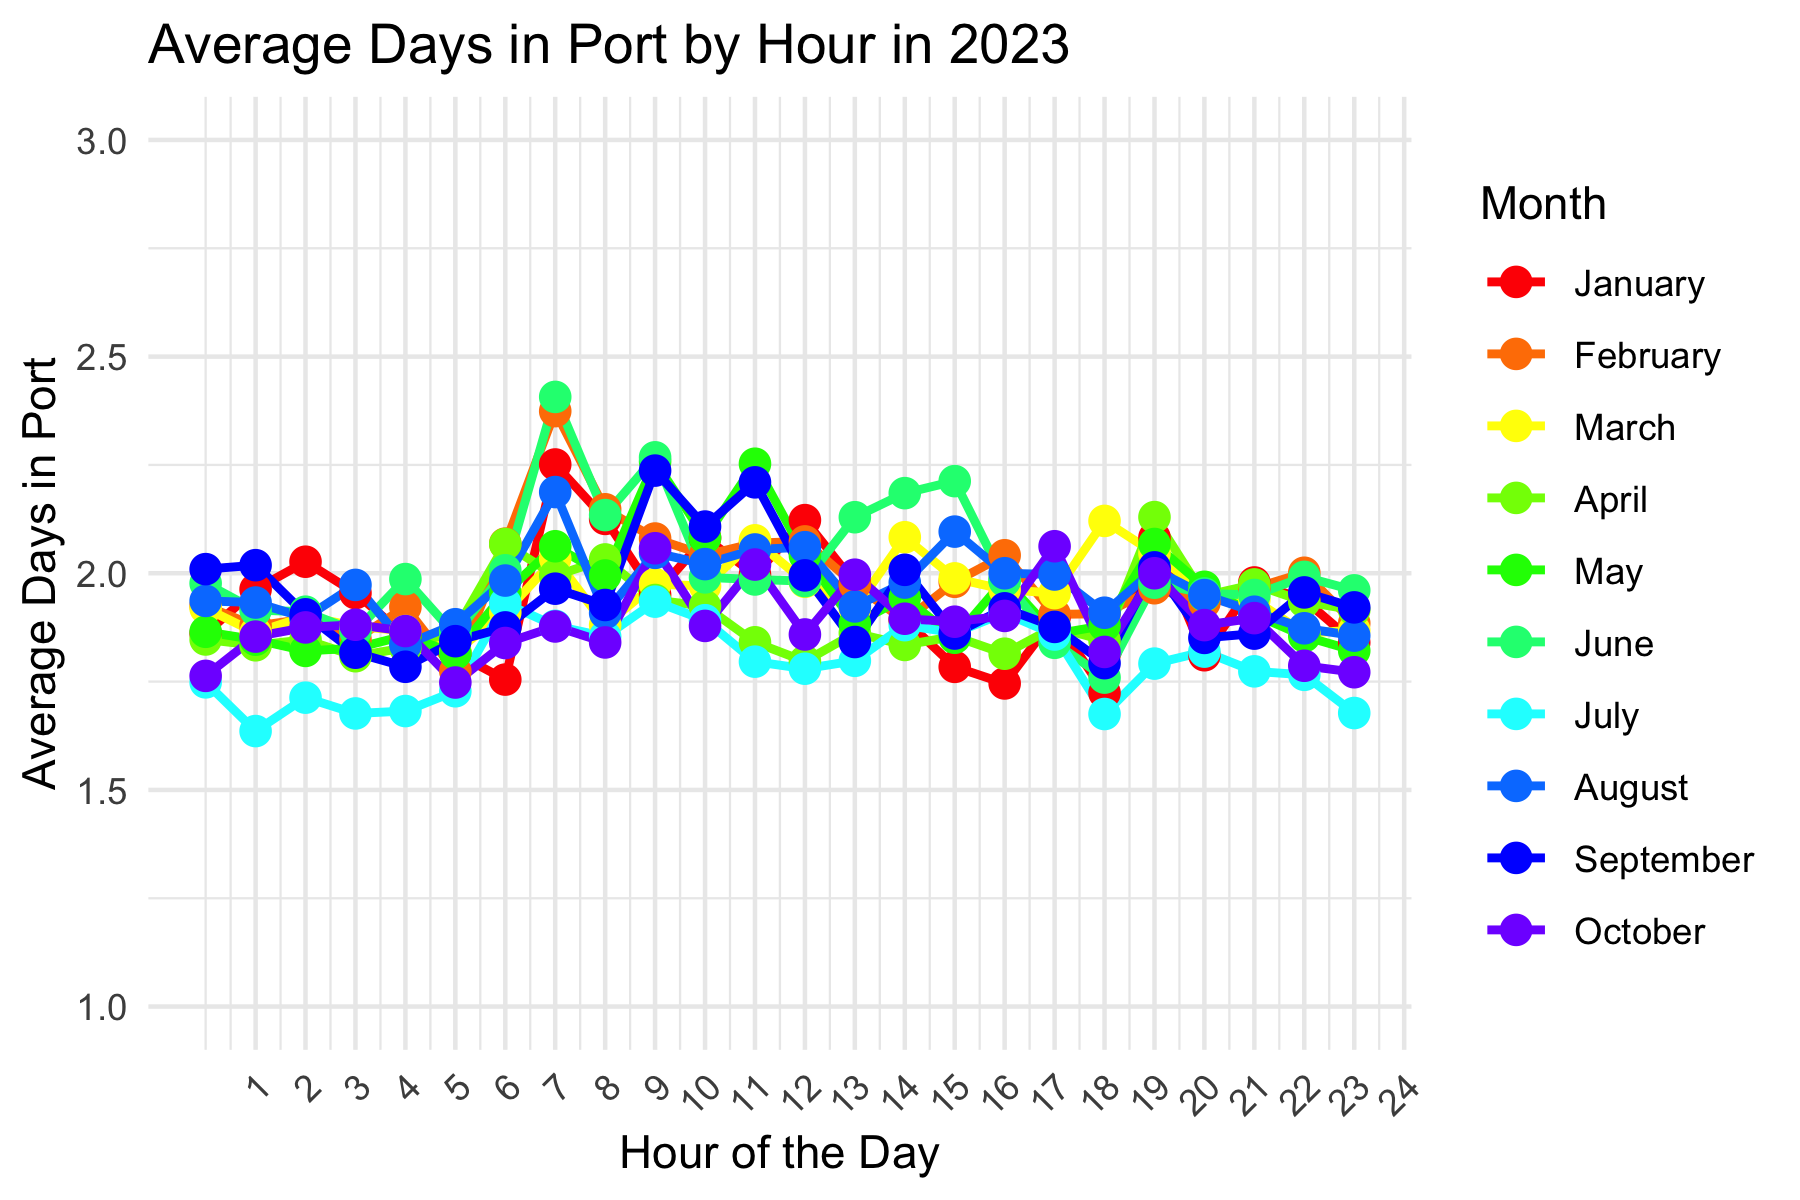
\includegraphics[width=0.8\textwidth]{images/du_seven}
				\caption{Average days in port by arrival hours per month}
				\label{fig:hourly_arrivals}
			\end{figure}
			Figure \ref{fig:hourly_arrivals} shows, in an hourly analysis of container and their dwell
			times throughout 2023 shows patterns that could be valuable for predictive modeling. The most notable
			feature is a consistent peak in dwell times during the morning (7:00-8:00 AM), where containers typically
			stay 2.2-2.4 days. This morning peak is particularly pronounced in June, which shows the highest dwell
			times during these hours. There is a cycle that starts with relatively stable dwell times of 1.8-2.0 days
			during early morning hours (1-5 AM), followed by the sharp morning peak (6-9 AM), then maintaining slightly
			elevated but more stable times during midday (10-15), before gradually declining through the afternoon and
			evening hours (16-24). These seasonal variations are evident, with summer months (June-August) having more
			volatility in dwell times, while July consistently shows lower overall dwell times than other months.
			Winter months (January-February) exhibit more consistent patterns with less variation. These interactions
			between arrival hour and month seem to be a possible factor in determining dwell times, as evidenced by
			the varying patterns across different months at specific hours. This suggests that both the hour of
			arrival and the month and their interaction term should be considered features for the predictive model.
			\\
			\\
			\begin{figure}[ht]
				\centering
				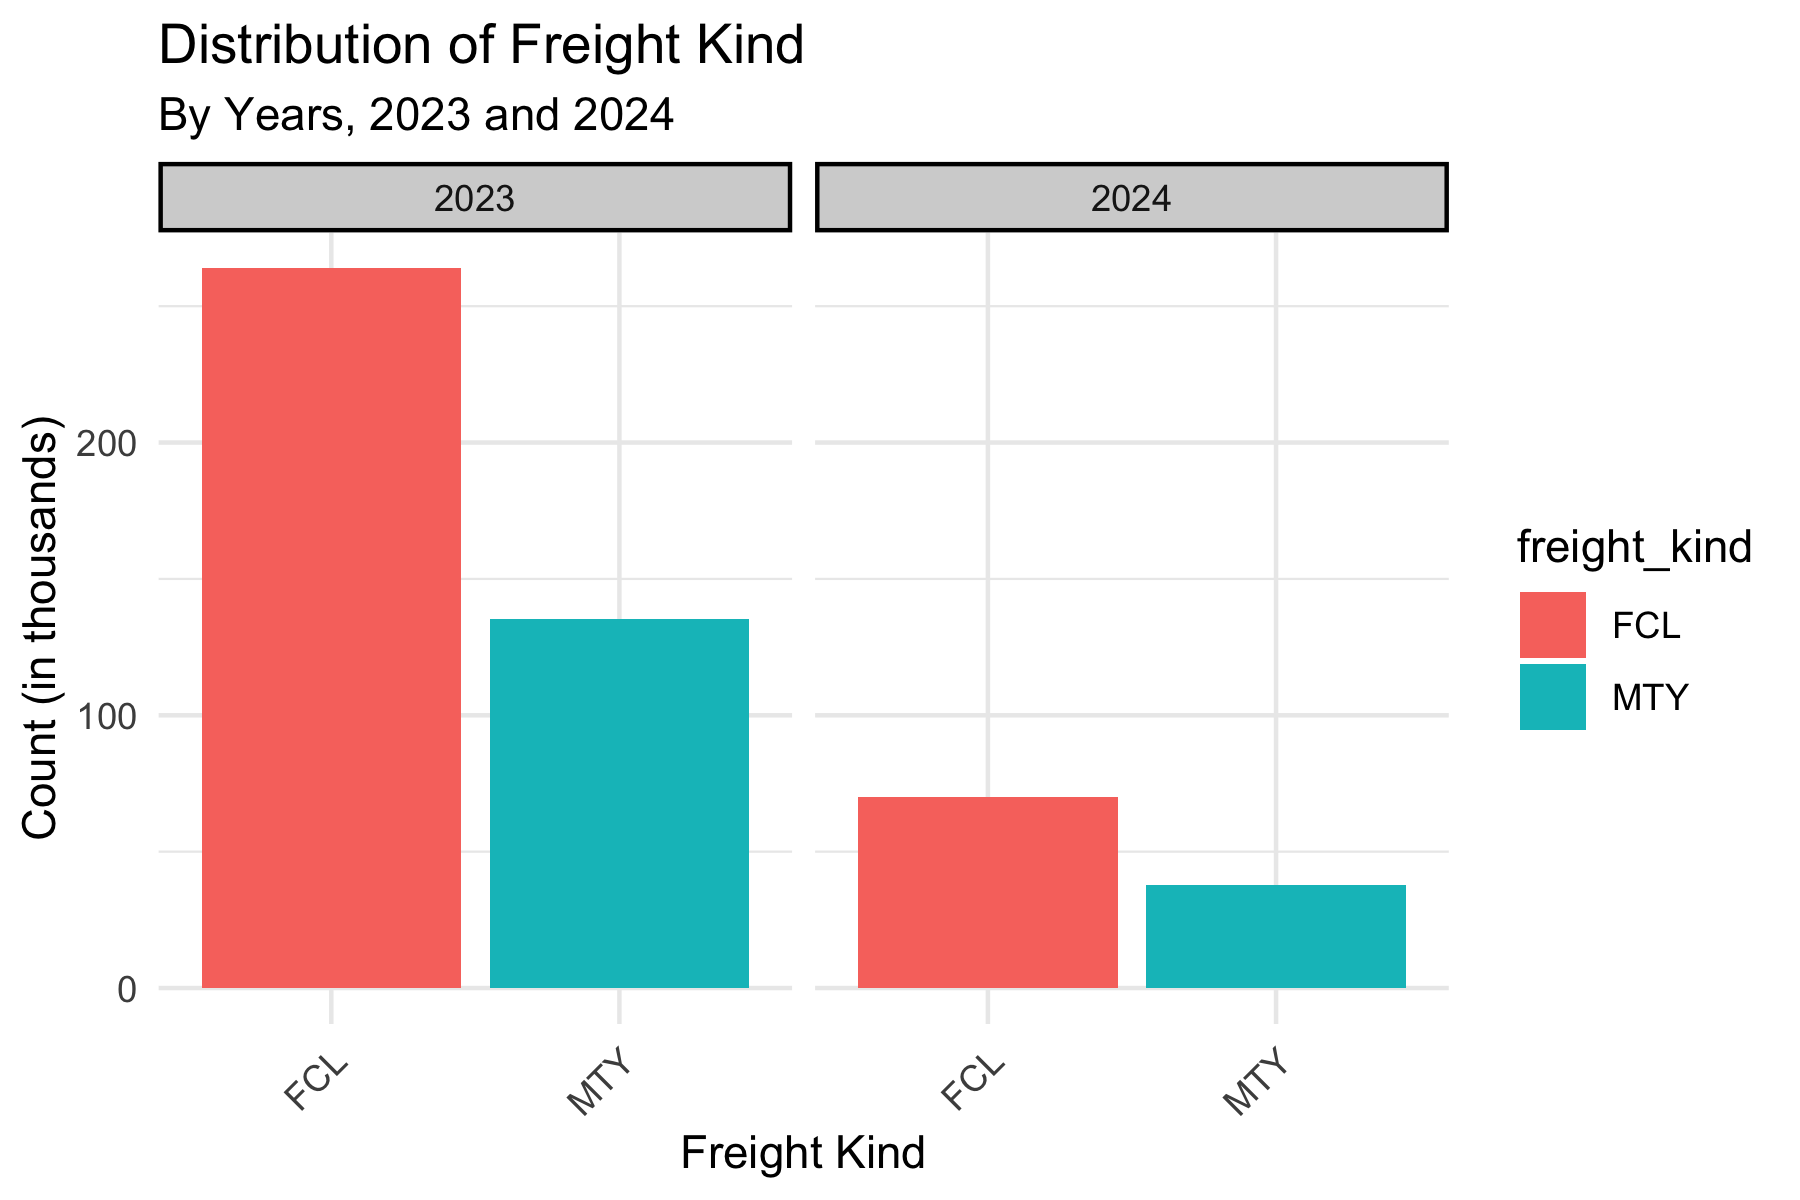
\includegraphics[width=0.5\textwidth]{images/du_four}
				\caption{Distribution of container by Freight Kind}
				\label{fig:freigh_kind_distribution}
			\end{figure}

			\begin{figure}[ht]
				\centering
				\begin{minipage}{0.5\textwidth}
					\centering
					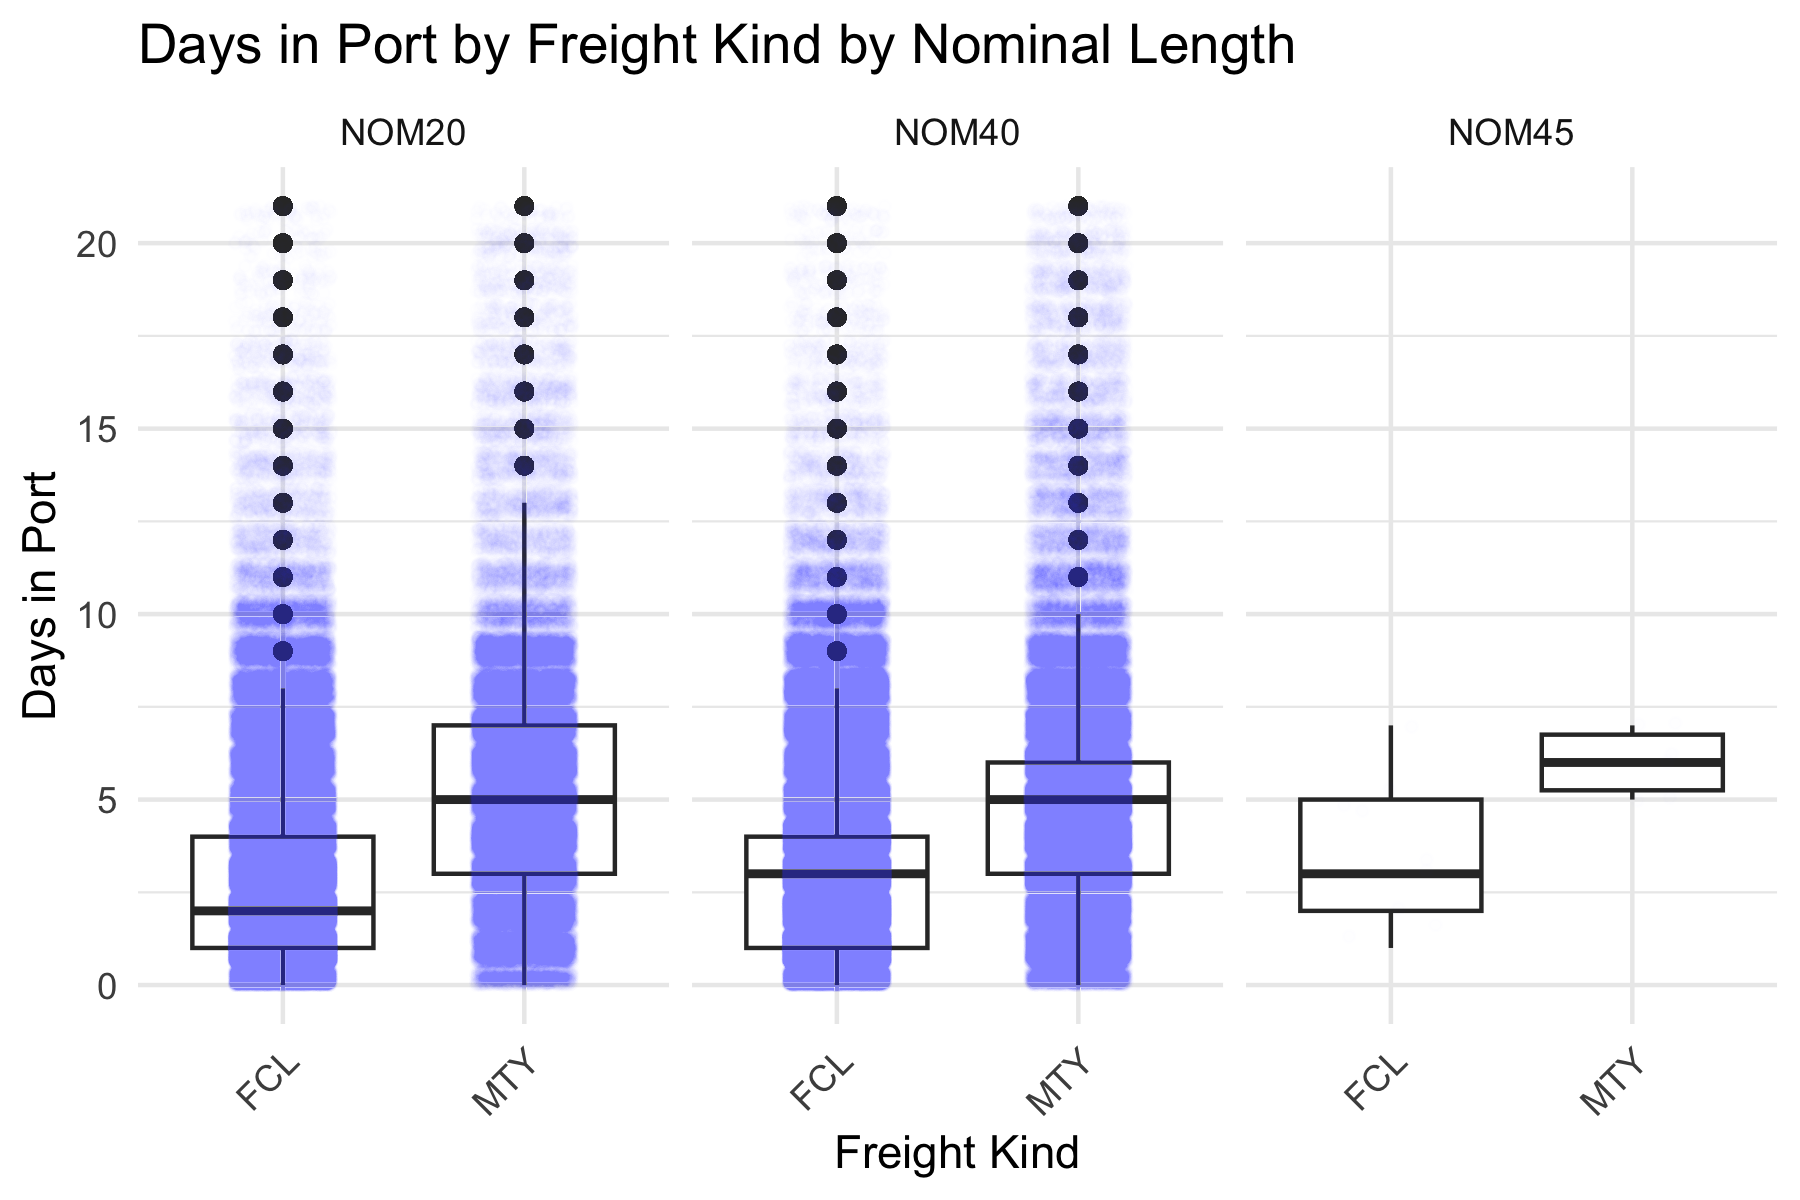
\includegraphics[width=\textwidth]{images/du_three}
					\caption{Freight kind vs size}
					\label{fig:freigh_kind_and_nominal_length}
				\end{minipage}%
				\hfill
				\begin{minipage}{0.5\textwidth}
					\centering
					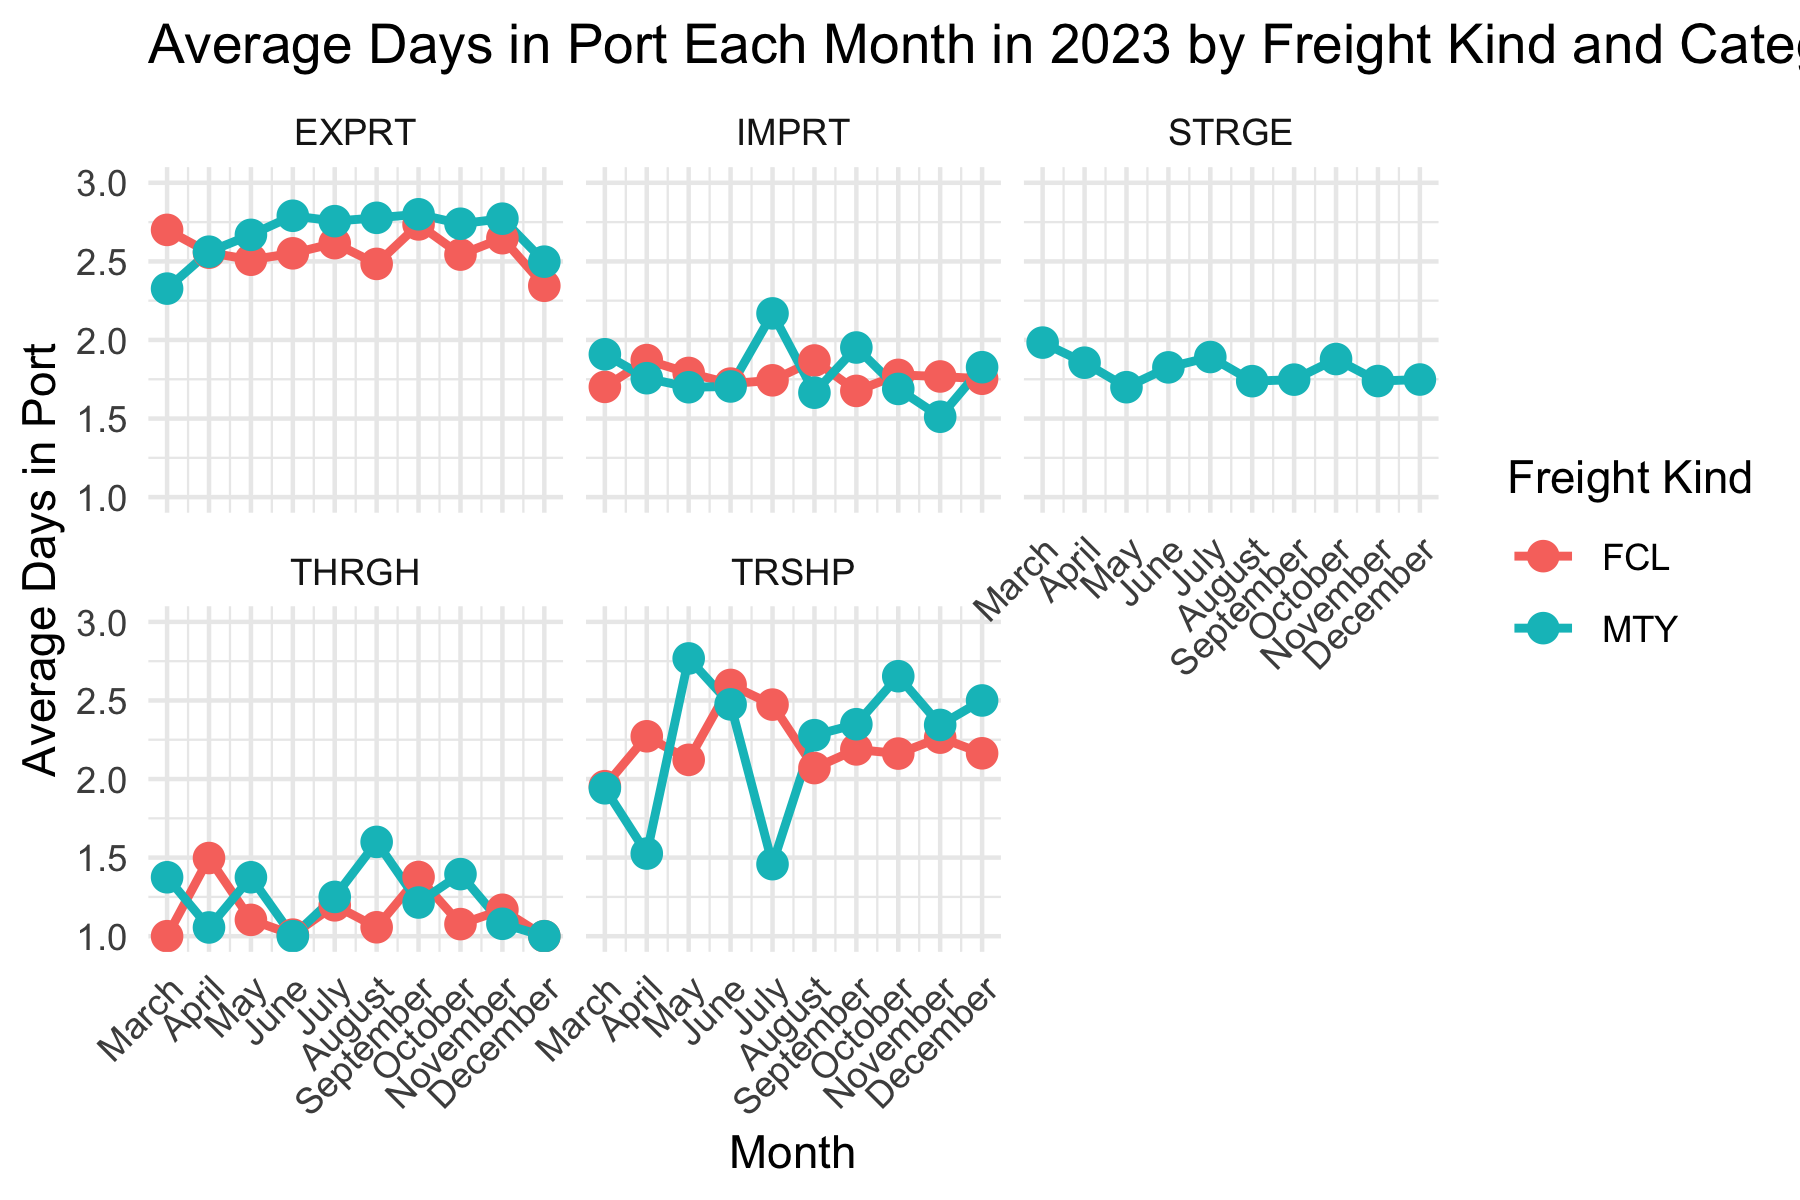
\includegraphics[width=\textwidth]{images/du_two}
					\caption{Month vs freight kind}
					\label{fig:category_freiht_kind_and_month}
				\end{minipage}
			\end{figure}

			Several insights about freight characteristics and their potential impact on dwell times could be valuable
			features for predictive modeling. Looking at figure \ref{fig:freigh_kind_distribution}
			, the data shows two main types of freight: FCL (Full Container Load) and MTY (Empty) containers, with FCL
			having higher counts in both 2023 and 2024.
			From figure \ref{fig:freigh_kind_and_nominal_length}
			, when examining dwell times across different nominal lengths (NOM20, NOM40, NOM45), MTY containers
			consistently show longer average dwell times than FCL containers, with the median dwell time for MTY
			containers being approximately five days compared to 2-3 days for FCL across all container sizes,
			suggesting that container type (FCL vs MTY) and nominal length are important predictive features. Figure
			\ref{fig:category_freiht_kind_and_month} breaks down the operational types (EXPRT,
			IMPRT, STRGE, THRGH, TRSHP) by month, revealing distinct patterns: EXPRT containers show consistently
			higher dwell times (around 2.5-3 days) with slight monthly variation, while THRGH (through) containers
			have the lowest dwell times (around 1-1.5 days). TRSHP (transshipment) containers show the highest
			variability in dwell times, suggesting that category is a crucial predictor. The interaction between
			freight kind and category type also appears significant, as shown in figure
			\ref{fig:category_freiht_kind_and_month}, where FCL and MTY containers show different
			patterns within each operational category. For a predictive model, key features should include freight
			kind (FCL/MTY) as shown in figure \ref{fig:freigh_kind_distribution}, container size (nominal length)
			from figure \ref{fig:freigh_kind_and_nominal_length}, category (EXPRT/IMPRT/STRGE/THRGH/TRSHP) from
			figure \ref{fig:category_freiht_kind_and_month}, and their possible interactions.
			\\
			\\
			\begin{figure}[ht]
				\centering
				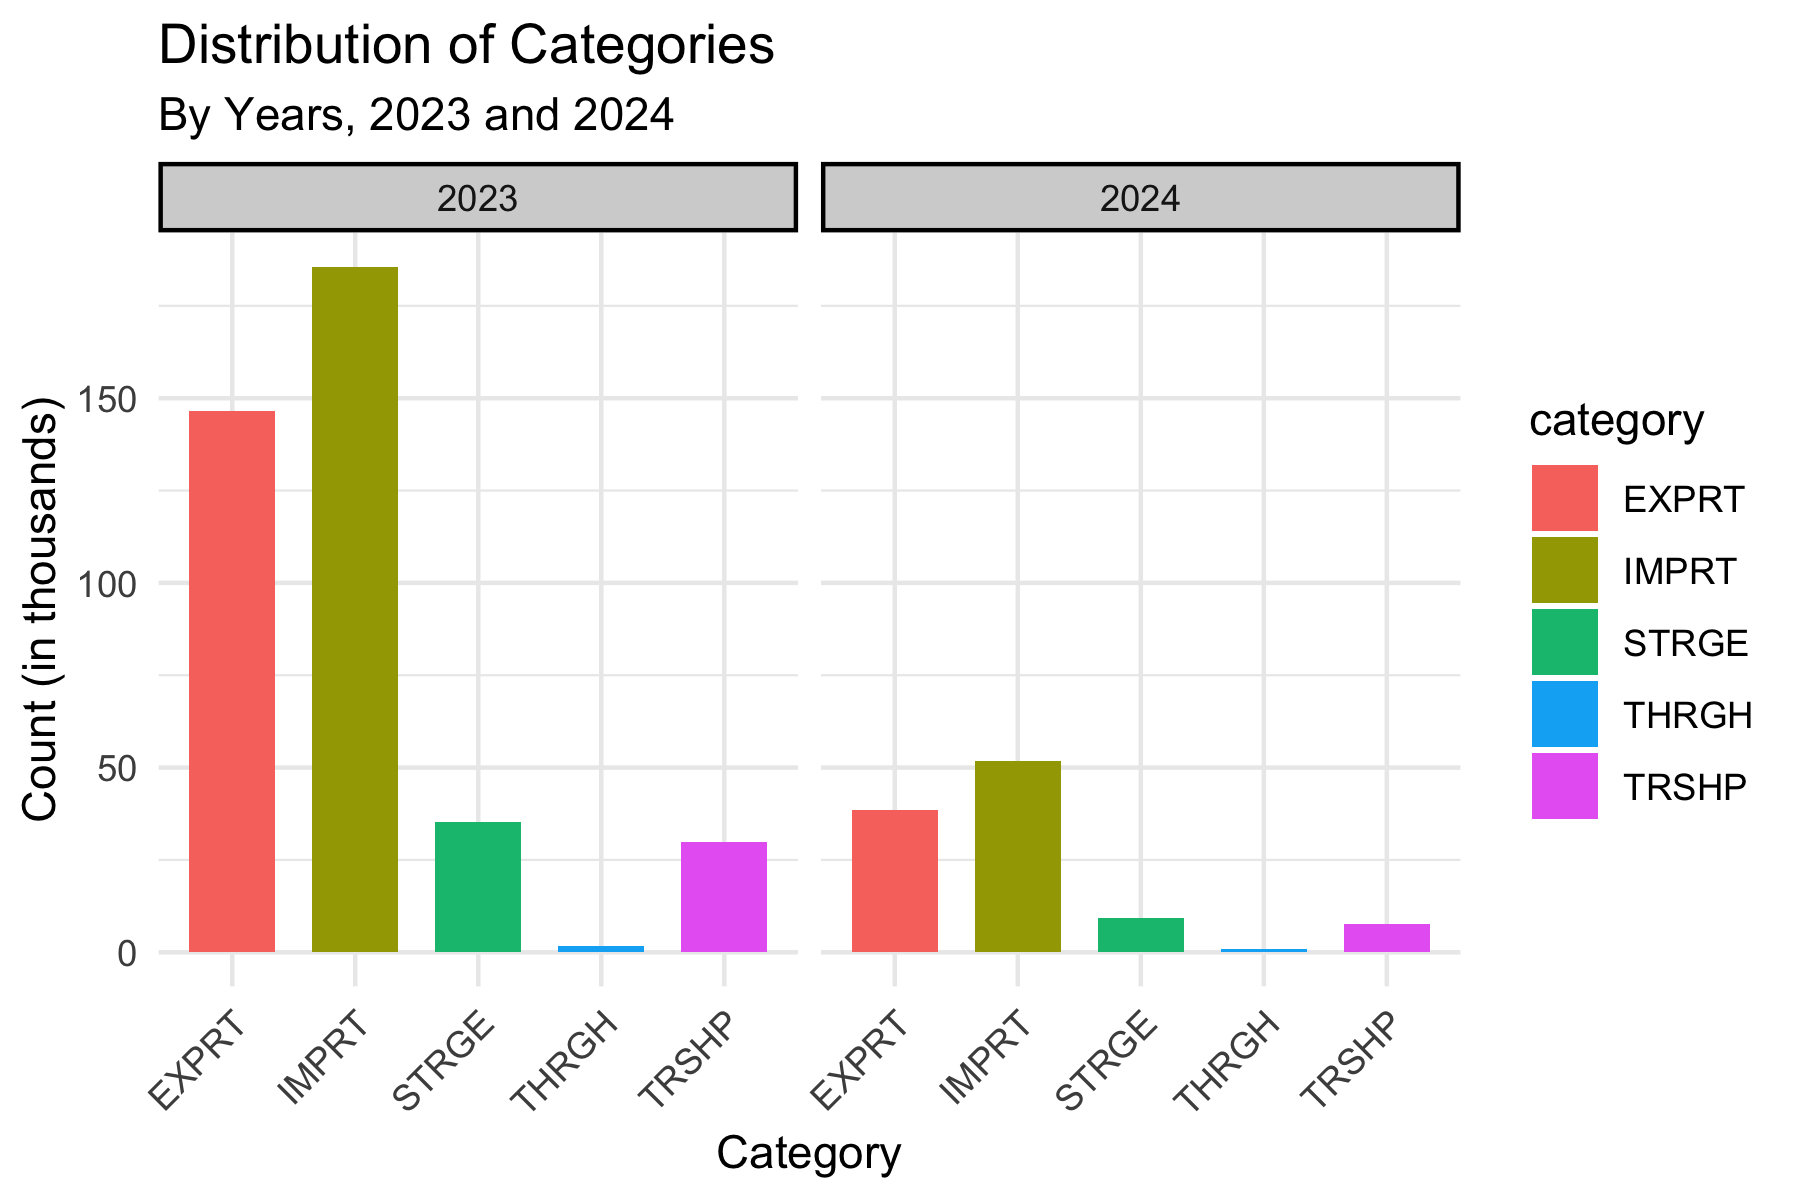
\includegraphics[width=0.5\textwidth]{images/du_five}
				\caption{Distribution of categories}
				\label{fig:category_distribution}
			\end{figure}
			\begin{figure}[ht]
				\centering
				\begin{minipage}{0.5\textwidth}
					\centering
					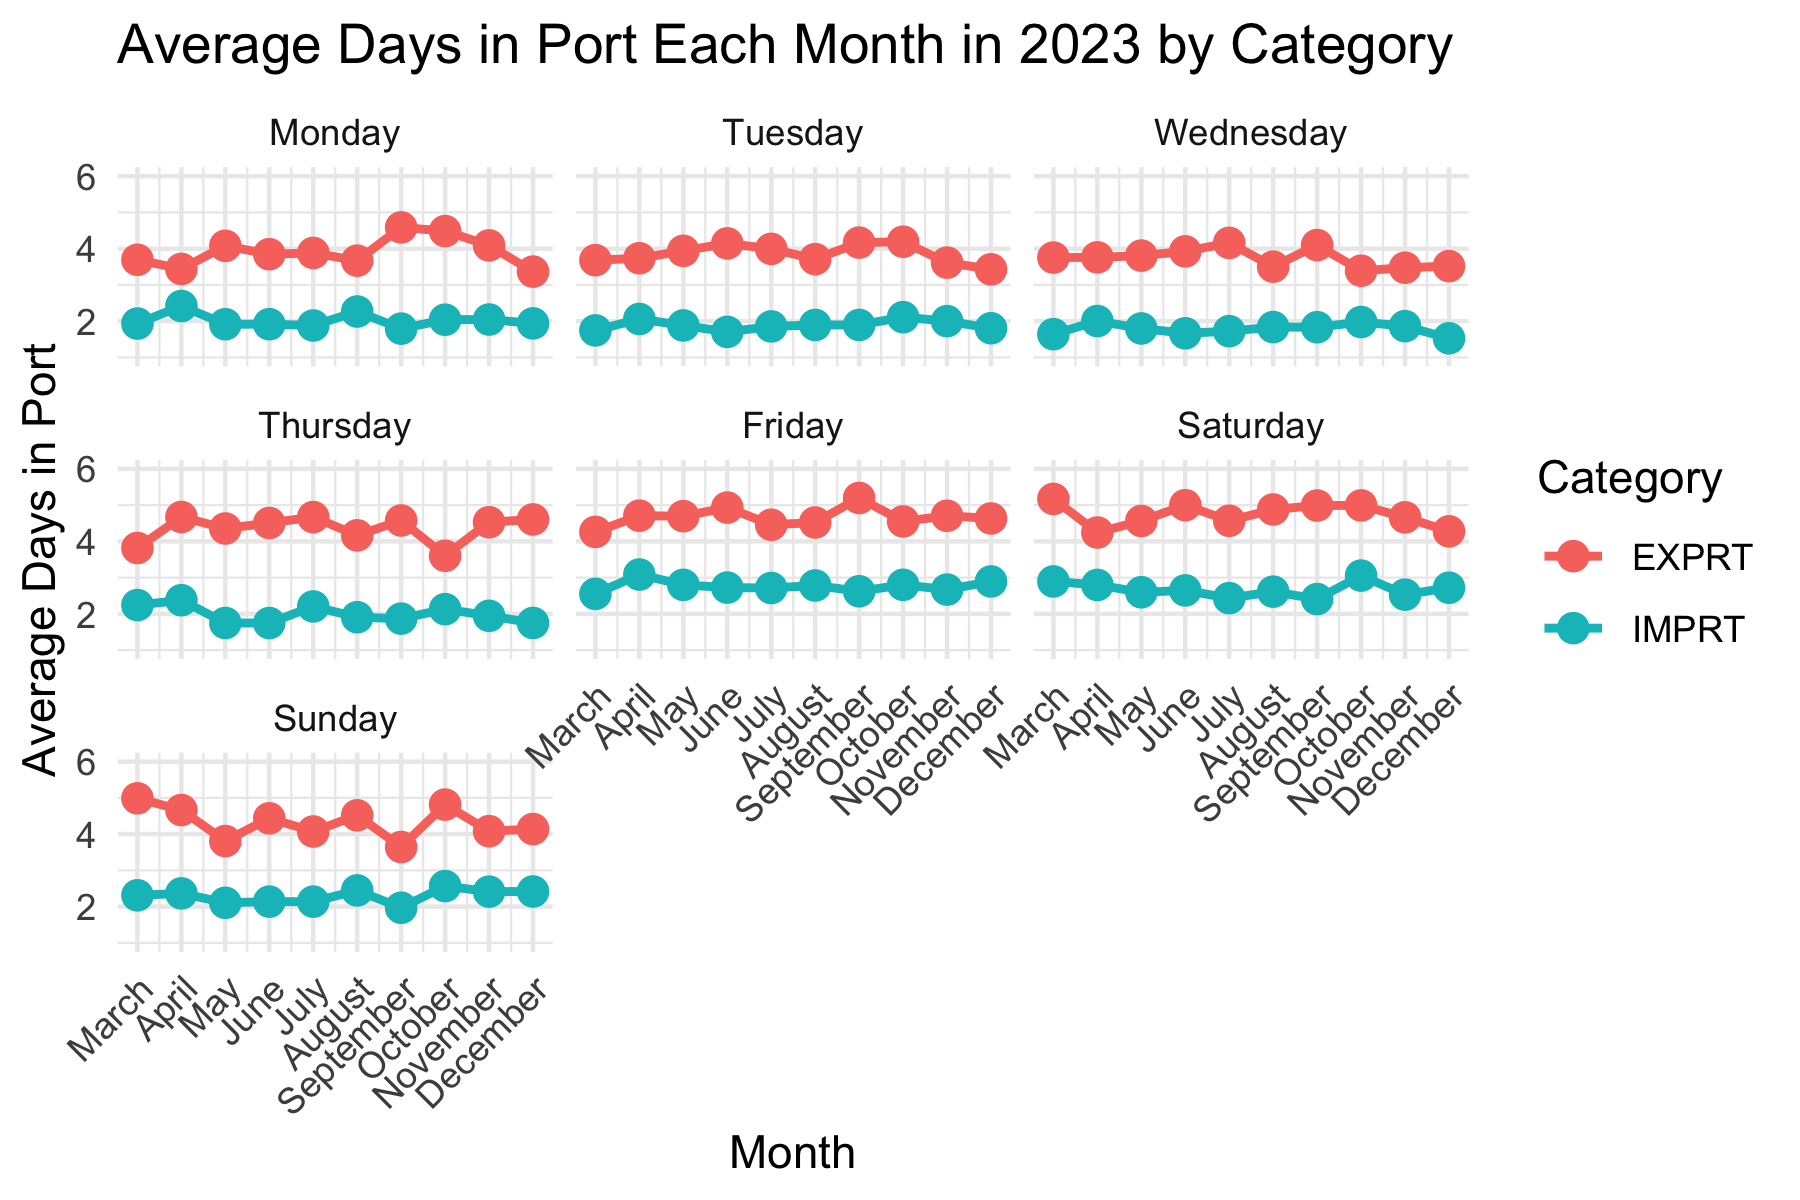
\includegraphics[width=\textwidth]{images/du_one}
					\caption{Month, day, and category}
					\label{fig:dwell_month_day_category}
				\end{minipage}%
				\hfill
				\begin{minipage}{0.5\textwidth}
					\centering
					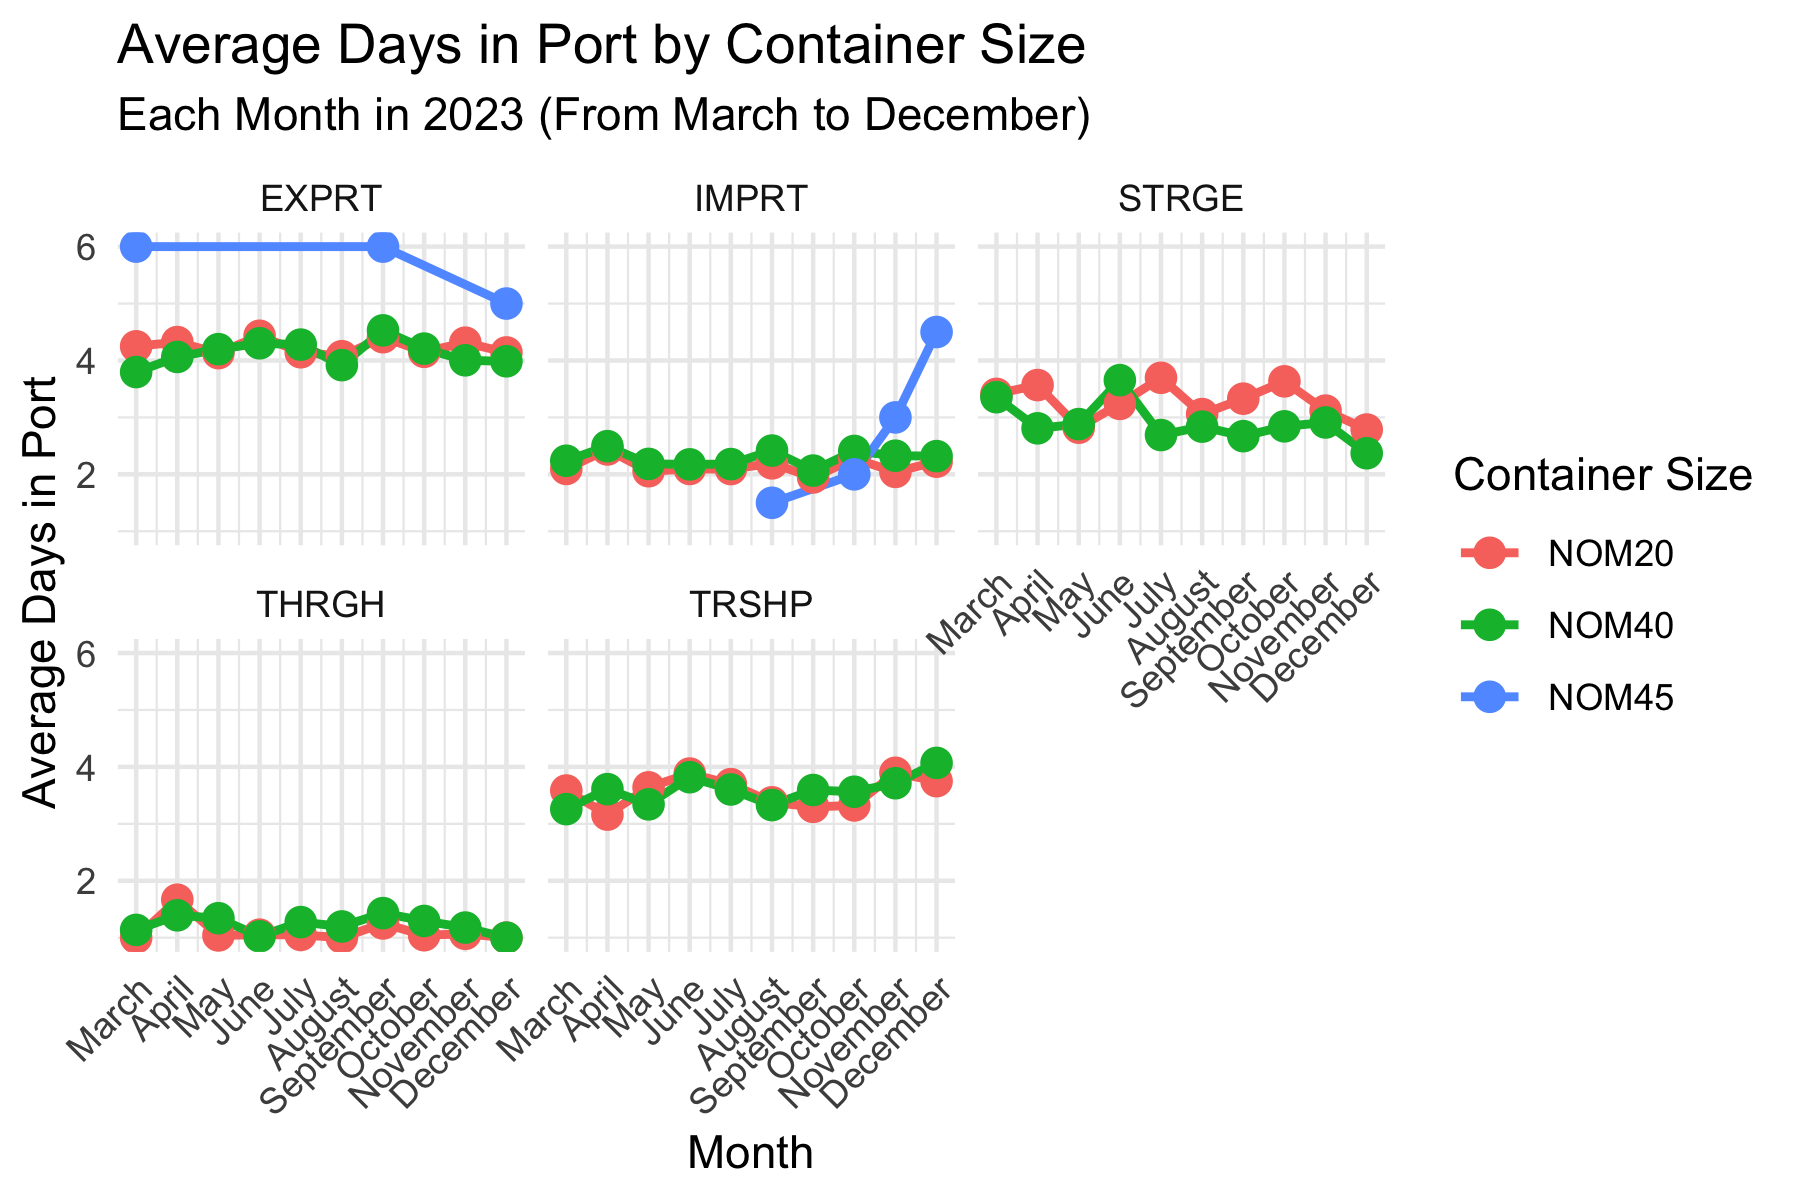
\includegraphics[width=\textwidth]{images/du_six}
					\caption{Month, category, and size}
					\label{fig:dwell_month_category_size}
				\end{minipage}
			\end{figure}
			Additionally, for categories, figure \ref{fig:dwell_month_day_category} shows patterns where export (
			EXPRT) containers consistently show higher dwell times (around 4 days) compared to import (IMPRT)
			containers (around 2 days) across all days of the week and the year. There is slight variation across
			weekdays, with Friday and Saturday showing marginally higher dwell times for both categories. Figure
			\ref{fig:category_distribution} shows the volume distribution across different operational categories,
			with IMPRT having the highest volume, followed by EXPRT in 2023 and 2024, though both show significant
			decreases in 2024. STRGE, THRGH, and TRSHP have notably lower volumes. figure
			\ref{fig:dwell_month_category_size} demonstrates how container size impacts dwell times across different
			operational categories - NOM45 containers show distinctly higher dwell times in EXPRT operations (around
			6 days) than NOM20 and NOM40 (around 4 days). In IMPRT operations, all container sizes show similar
			dwell times (around 2 days), while TRSHP shows more variability across container sizes. For predictive
			modeling, key features should include the day of the week (shown important in figure
			\ref{fig:dwell_month_day_category}), operational category (EXPRT/IMPRT/STRGE/THRGH/TRSHP as shown in
			Figure \ref{fig:category_distribution}), container size (NOM20/40/45 from figure
			\ref{fig:dwell_month_category_size}). The temporal patterns across days of the week (figure
			\ref{fig:dwell_month_day_category}) suggest that day-of-week and weekend/weekday indicators would be
			helpful to features.
			\\
			\\
			This analysis uncovered some patterns that influence how long containers stay in port. The timing of
			container arrivals matters significantly - there is a clear morning peak around 7-8 AM when containers tend
			to stay longer, and this varies across different days of the week and seasons. The category type plays a
			significant role: export containers consistently stay about twice as long as imports (4 days versus 2
			days), regardless of when they arrive. We have also seen empty containers generally stay longer than full
			ones, and larger containers (especially 45-footers) tend to need more time in port, particularly for
			exports. Given these findings, a predictive model should focus on three main aspects: when containers
			arrive (time of day, day of week, and season), what kind of operation they are part of (export, import,
			storage, etc.), and their physical characteristics (size and whether they are full or empty). Building
			models upon those found features could make it possible to develop solid predictors for how long
			containers will stay in port.

	\chapter{Methodology}%    \chapter{}  = level 1, top level


	\section{Problem Definition}
		The main challenge for optimizing container yard operations at the Ports of Auckland was predicting dwell times
		to support placement decisions.
		\\
		\\
		Predicting the exact number of days for each container was the first approach. Using classifier models with the
		selected features, predicting how many days each container would stay in the port was set as a target. The
		metrics in the models, especially accuracy, were low.
		\\
		\\
		The variance in the predicted days was tremendous. Some similar-character containers were taken out daily while
		others stuck around for weeks. There needed to be a clear pattern for the classifier to generate acceptable
		predictions.
		\\
		\\
		Rather than predicting an exact number of days, a range of days was a better approach improving the results.
		Having more than one range of days allows port managers to have options to make decisions, balancing prediction
		accuracy with operational utility.


	\section{Dataset Strategy and Model Evaluation}

		The experimental approach employs a temporal split strategy to ensure robust model development and realistic
		performance evaluation. As detailed in Table~\ref{tab:dataset-split}
		, 2023 dataset will be used for the development phase, allocating 80\% for training and 20\%
		for cross-validation. This split enables thorough model tuning and hyperparameter optimization while
		maintaining statistical validity. For final evaluation, 2024 dataset will be used as an unseen test
		set, providing a true assessment of how the models perform on future data. This temporal separation is
		crucial as it mirrors real-world conditions where models must predict outcomes for future periods.

		\begin{table}[ht]
			\centering
			\begin{tabular}{|l|c|l|}
				\hline
				\textbf{Time Period} & \textbf{Data Split} & \textbf{Purpose}                             \\
				\hline
				\multirow{2023}          & 80\%                & Training Set: Model development and fitting  \\
				& 20\%                & Validation Set: Cross-validation and tuning  \\
				\hline
				2024                     & 100\%               & Testing Set: Final evaluation on unseen data \\
				\hline
			\end{tabular}
			\caption{Dataset Split Strategy for Model Development and Evaluation}
			\label{tab:dataset-split}
		\end{table}

		The development process begins with initial model training on the 2023 training set. Cross-validation
		techniques are employed during this phase to optimize model hyperparameters and assess performance
		stability. Once the bet models are selected and tuned, those final models will be evaluated over the 2024
		dataset. This approach provides a rigorous test of model generalization, as the evaluation data represents
		genuinely unseen future observations.


	\section{Selecting Time Range Categories and Classifiers}
		This research took a data-driven approach to identify an optimal set of ranges of days to predict dwell time.
		Iteratively, multiple time range configurations were tested to find groupings that allowed operational needs to
		be achieved and predictions with solid performance generated.
		\\
		\\
		The search for optimal time ranges involved systematically evaluating different bin configurations. Each
		configuration was tested across multiple machine learning algorithms to ensure the selected ranges would be
		robust across different modeling approaches. The goal was to find time ranges reflecting meaningful operational
		distinctions in container handling, provide sufficient data in each category for reliable model training, and
		enable predictive solid performance across different algorithms.
		\\
		\\
		Multiple models were fit, using the training set (table~\ref{tab:dataset-split}
		), to be evaluated based on their metrics in finding ranges of days and classifiers. The models and ranges
		with the best performance, evaluated by F1 Score, were chosen to follow the next step: prediction evaluation.
		\\
		\\
		Five classifiers were fitted initially: Random Forest, K-Nearest Neighbors, Logistic Regression, Gradient
		Boosting, and Naive Bayes (table~\ref{tab:model-type-counts}).

		\begin{table}[ht]
			\centering
			\begin{tabular}{|l|c|}
				\hline
				\textbf{Model Type} & \textbf{Models Fitted} \\
				\hline
				Gradient Boosting       & 64                     \\
				KNN                     & 64                     \\
				Logistic Regression     & 64                     \\
				Naïve Bayes             & 52                     \\
				Random Forest           & 64                     \\
				\hline
				\textbf{Grand Total}    & \textbf{308}           \\
				\hline
			\end{tabular}
			\caption{Number of Models Fitted by Type}
			\label{tab:model-type-counts}
		\end{table}

		Random Forest was a top performer (Table~\ref{tab:model-type-performance}) with an impressive 87.0\%
		F1 Score, showing remarkable consistency with its similar accuracy of 86.9\%
		, having the best overall balance between precision and recall.
		KNN's performance had the second place with 86.0\%
		F1 Score close to Random Forest in both metrics. More powerful classifier than initially expected.
		Gradient Boosting and Logistic Regression performed adequately but notably below the top two. Gradient
		Boosting achieved 77.0\% F1 Score while Logistic Regression close behind at 76.0\%
		. Naïve Bayes underperformed with just a 5.0\%
		F1 Score, clearly not suitable for this specific prediction task.

		\begin{table}[ht]
			\centering
			\begin{tabular}{|l|c|c|}
				\hline
				\textbf{Model Type} & \textbf{Max F1 Score} & \textbf{Max Test Accuracy} \\
				\hline
				Random Forest           & 87.0\%                & 86.9\%                     \\
				KNN                     & 86.0\%                & 86.3\%                     \\
				Gradient Boosting       & 77.0\%                & 78.7\%                     \\
				Logistic Regression     & 76.0\%                & 76.7\%                     \\
				Naïve Bayes             & 5.0\%                 & 9.6\%                      \\
				\hline
			\end{tabular}
			\caption{Model Type Performance Metrics}
			\label{tab:model-type-performance}
		\end{table}

		The models selected with appropriate metrics were Random Forest, KNN, Gradient Boosting and Logistic
		Regression.

		After being sure that there were models that performed as expected, the next step was selecting the
		group of range to be used in the model. Those models were fitted with multiple groups of ranges to allow a
		posterior analysis based on F1-Score values, making sure that at least any range was significant.

		\subsection{Finding Ranges and Defining data scaling strategy}

			Some groups of ranges were over 80\% (table~\ref{tab:bins-ranges})
			of accuracy and F1-Score. As there were appropriate thresholds of metrics overtaken, the analysis
			continued over classifiers to check which ranges were shared among them. The best ones were kept for
			posterior analysis.

			\begin{table}[ht]
				\centering
				\small
				\begin{tabular}{|l|c|c|c|}
					\hline
					\textbf{Bins Ranges} & \textbf{Models Fitted} & \textbf{Max Test Accuracy}
					& \textbf{Max F1 Score}
					\\
					\hline
					{[}0, 3, 10, 21{]} & 20 & 79\% & 79.0\% \\
					{[}0, 3, 11, 21{]} & 20 & 80\% & 80.0\% \\
					{[}0, 3, 12, 21{]} & 20 & 80\% & 80.0\% \\
					{[}0, 3, 9, 21{]}  & 20 & 78\% & 77.0\% \\
					{[}0, 4, 10, 21{]} & 16 & 83\% & 82.0\% \\
					{[}0, 4, 11, 21{]} & 16 & 83\% & 83.0\% \\
					{[}0, 4, 12, 21{]} & 20 & 84\% & 83.0\% \\
					{[}0, 4, 9, 21{]}  & 16 & 81\% & 81.0\% \\
					{[}0, 5, 10, 21{]} & 20 & 85\% & 85.0\% \\
					{[}0, 5, 11, 21{]} & 20 & 85\% & 85.0\% \\
					{[}0, 5, 12, 21{]} & 20 & 86\% & 85.0\% \\
					{[}0, 5, 9, 21{]}  & 20 & 84\% & 84.0\% \\
					{[}0, 6, 10, 21{]} & 20 & 86\% & 86.0\% \\
					{[}0, 6, 11, 21{]} & 20 & 87\% & 86.0\% \\
					{[}0, 6, 12, 21{]} & 20 & 87\% & 87.0\% \\
					{[}0, 6, 9, 21{]} & 20 & 86\% & 85.0\%
					\\
					\hline
					\textbf{Total} & \textbf{308} & \textbf{} & \textbf{}
					\\
					\hline
				\end{tabular}
				\caption{Ranges and Max possible F1-Scores and accuracy by Fitted Models}
				\label{tab:bins-ranges}
			\end{table}

			Additionally, each model and range was also trained using a combination of techniques, including
			scaling via SMOTE (Synthetic Minority Over-sampling Technique) and stratification based on weekly and
			monthly. The goal was to explore whether scaling or stratification would improve the model’s ability to
			handle imbalanced data effectively.

			\begin{table}[ht]
				\centering
				\small
				\begin{tabular}{|l|c|c|c|c|c|}
					\hline
					\textbf{Range} & \textbf{F1 Score} & \textbf{Precision} & \textbf{Recall} & \textbf{Scaled}
					& \textbf{Stratified}
					\\
					\hline
					\multicolumn{6}{|l|}{\textbf{[0, 4, 10, 21]}} \\
					\hline
					& 0.81 & 0.81 & 0.81 & False & False \\
					& 0.81 & 0.81 & 0.81 & False & True  \\
					& 0.81 & 0.81 & 0.81 & True  & False \\
					& 0.81 & 0.81 & 0.81 & True  & True  \\
					& 0.81 & 0.82 & 0.81 & True  & False \\
					& 0.82 & 0.82 & 0.83 & False & False \\
					& 0.82 & 0.83 & 0.83 & False & True  \\
					\hline
					\multicolumn{6}{|l|}{\textbf{[0, 4, 11, 21]}} \\
					\hline
					& 0.81 & 0.82 & 0.82 & True  & True  \\
					& 0.82 & 0.82 & 0.82 & False & False \\
					& 0.82 & 0.82 & 0.82 & False & True  \\
					& 0.82 & 0.82 & 0.82 & True  & False \\
					& 0.82 & 0.83 & 0.82 & True  & False \\
					& 0.83 & 0.83 & 0.83 & False & False \\
					& 0.83 & 0.83 & 0.83 & False & True  \\
					\hline
					\multicolumn{6}{|l|}{\textbf{[0, 4, 12, 21]}} \\
					\hline
					& 0.81 & 0.82 & 0.80 & True  & True  \\
					& 0.82 & 0.82 & 0.82 & False & False \\
					& 0.82 & 0.82 & 0.82 & False & True  \\
					& 0.82 & 0.82 & 0.82 & True  & False \\
					& 0.82 & 0.82 & 0.82 & True  & True  \\
					& 0.83 & 0.83 & 0.82 & True  & False \\
					& 0.83 & 0.84 & 0.84 & False & False \\
					& 0.83 & 0.84 & 0.84 & False & True  \\
					\hline
				\end{tabular}
				\caption{Performance Metrics by Range Under Different Conditions}
				\label{tab:bins-performance-conditions}
			\end{table}


			After multiple iterations and testing (table~\ref{tab:bins-performance-conditions}
			), regarding data scaling and stratification, the metrics in each approach did not lead to any significant
			improvements and, in some cases, resulted in worse performance. Consequently, it was determined that
			neither scaling nor stratification was beneficial for this particular dataset, and these techniques
			were not applied in the final model.
			\\
			\\
			Given the presence of attractive ranges and classifiers and the fact that no stratification or scaling was
			required, a group of ranges was selected. The optimal group, identified as the best across all the
			configurations, consisted of 0-3 days, 4-11 days, and 12+ days ([0, 4, 12, 21]). These groups of ranges
			provided solid performance, an acceptable data distribution (fig. \ref{fig:class_ranges_distribution}
			) while allowing the defined ranges to be good enough to establish stacking strategies for the
			port.

			\begin{figure}[ht]
				\centering
				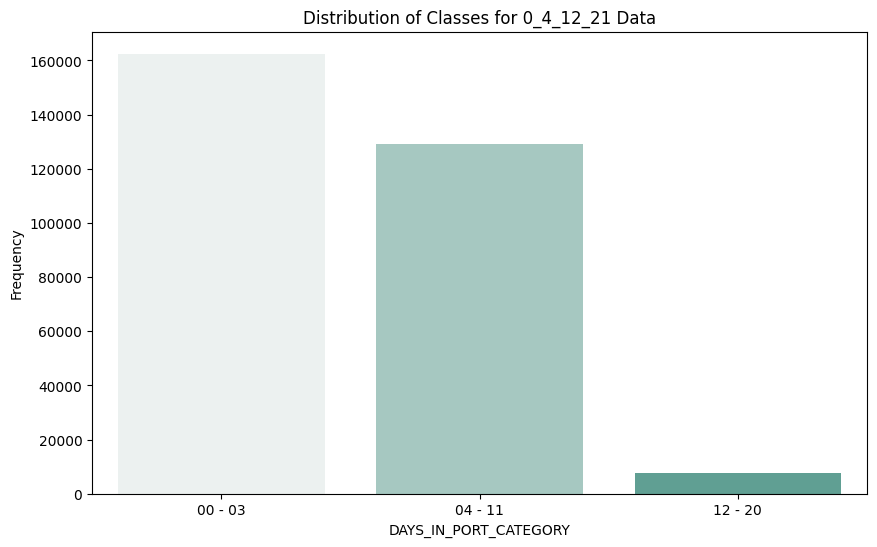
\includegraphics[width=0.5\textwidth]{images/ClassRangesDistribution}
				\caption{Ranges Distribution Labels}
				\label{fig:class_ranges_distribution}
			\end{figure}

		\subsection{Class Imbalance Analysis}

			The distribution of container dwell times are imbalanced across the three categories (fig.~
			\ref{fig:class_ranges_distribution}
			). The largest group, the short-term stays (0-3 days), has around 160,000 containers. For
			Medium-term stays (4-11 days), there are about 130,000 containers. For the smallest group, long-term
			stays (12-20 days), there are significantly fewer containers, with only 10,000 units representing a small
			portion of the overall data.

		\subsection{Selecting the Metric: F1 Score}

			\subsubsection{Addressing the Imbalance:}
				Ranges evaluated were more common than others (Figure~
				\ref{fig:class_ranges_distribution}
				), which led to an imbalanced evaluation, generating a wrong sense of good predictions. The accuracy
				metric misled these models' results by predicting the most frequent classes. F1-Score corrected this,
				providing a more appropriate understanding of the real performance.
				\\
				\\
				Due to this imbalanced distribution, the F1 Score provides a handy evaluation metric. Since accuracy
				could be misleading, with short and medium-term stays making up more than 95\%
				of cases, the F1 Score offers a more balanced assessment by considering precision and recall.
				Addressing imbalance with a proper metric is essential because, in port operations, incorrectly
				predicting a longer stay (false positives) or failing to identify a long-term stay (false
				negatives) can result in inefficient container placement and higher rehandling costs. The F1
				Score’s sensitivity to both error types helps prevent models from appearing highly accurate by
				predicting the most common stay categories. Long-term stays are less frequent but impact yard
				management and resource allocation for the longer term; this is why the F1 Score is
				particularly valuable. The balance provided by the F1 Score fits well with the practical needs of port
				operations, providing accurate prediction evaluation across all dwell time categories, which is
				essential for efficient yard optimization.

			\subsubsection{Balancing Precision and Recall (Trade-off):}
				The F1 score is widely recognized for combining precision (proportion of true positive predictions
				among all positive predictions) and recall (proportion of true positive predictions among all actual
				positives).
				\\
				\\
				Identifying the correct range and minimizing the misclassifications was essential because the cost of
				misclassification was high. F1-score evaluates false positives (incorrectly assigning a range) and
				false negatives (failing to detect the correct range).


	\section{Model Refinement and Optimization}

		After selecting the classifiers, a metric, and defining their parameter ranges, they were fine-tuned to enhance
		performance. GridSearchCV was employed with 5-fold cross-validation to identify the optimal hyperparameters for
		each model. This process utilized 80\% of the 2023 data for training, with the remaining 20\%
		reserved for evaluation.

		\subsection{The Scoring Metric: Weighted F1 Score}

			Weighted F1 score was used for optimization metric during the tuning process, a choice driven by the
			imbalanced nature of our three classes.
			\\
			\\
			Unlike a simple F1 score, the weighted F1 score calculates metrics for each label and finds their average,
			weighted by the number of true instances for each label. This ensures that the performance of smaller
			classes is not overshadowed by larger classes.
			\\
			\\
			The three classes were imbalanced. The weighted F1 score offers an interpretable single metric that
			summarizes performance across all of them while respecting their different sizes. This approach led to more
			robust and reliable models that can effectively handle the class distribution in our dataset.

		\subsection{The hyperparameters}

			Each model was tuned with a set of hyperparameters to optimize its performance. The hyperparameters, as
			shown in Appendix~\ref{sec:hyperparameters}
			, were selected based on the models' characteristics and the nature of the dataset. The tuning
			process aimed to identify the best combination of hyperparameters that would maximize the models'
			predictive power.
			Many models were evaluated based on each algorithm's complexity during the hyperparameter tuning
			process.
			Random Forest required fitting 864 models while tuning six hyperparameters, including parameters
			like
			n\_estimators, max\_
			depth, and bootstrap options. Gradient Boosting, being the most complex regarding tunable
			parameters, involved fitting 972 models across seven hyperparameters, such as learning rate, number
			of estimators, and tree-specific parameters. Logistic Regression was less complex, requiring 360
			models to be fitted while tuning five hyperparameters, including regularization strength and solver
			options. The simplest model in terms of tuning was K-Nearest Neighbors, which needed only 60 models
			to be fitted while optimizing three hyperparameters: the number of neighbors, weight function, and
			distance metric.

		\subsection{The Best Parameters}

			The best parameters were selected based on the weighted F1 score as shown in Appendix~
			\ref{sec:best_params}.
			\\
			\\
			For Random Forest the best parameters were max\_depth (20) and min\_samples\_
			leaf (2) limit the tree size while reducing overfitting and maintaining robust learning. Using max\_
			features as “sqrt” and 500 estimators ensures better generalization by creating diverse trees.
			\\
			\\
			Nearest Neighbors selected parameters were Manhattan distance makes the model less sensitive to outliers,
			while
			23 neighbors smooth the predictions. Distance-weighted voting emphasizes closer data points, improving
			local
			prediction accuracy.
			\\
			\\
			The best parameters for Gradient Boosting where a moderate learning rate (0.1) combined with a controlled
			max\_
			depth (5) helps to prevent overfitting. The choice of 500 estimators allows the model to build a strong
			ensemble
			and subsampling features (max\_features: “sqrt”) enhance generalization.
			\\
			\\
			Regarding Logistic Regression, the best parameters were C=1 and l2 penalty for regularization and newton-cg
			solver.

		\subsection{Analysis of Model Tuning Results}
			\begin{table}[ht]
				\centering
				\begin{tabular}{|l|c|c|c|}
					\hline
					\textbf{Model} & \textbf{Precision} & \textbf{Recall} & \textbf{F1-Score} \\
					\hline
					Random Forest       & 0.8397             & 0.8395          & 0.8368            \\
					K-Nearest Neighbors & 0.8349             & 0.8337          & 0.8308            \\
					Gradient Boosting   & 0.8061             & 0.8073          & 0.8035            \\
					Logistic Regression & 0.7521             & 0.7666          & 0.7581            \\
					\hline
				\end{tabular}
				\caption{Model Performance Metrics (Ordered by F1-Score)}
				\label{tab:model-metrics}
			\end{table}

			\textbf{Random Forest} was the best among the four models. It achieved a high F1-score of 0.8368,
			with precision (0.8397) and recall (0.8395) showing consistency across all classes.
			\\
			\\
			\textbf{K-Nearest Neighbors} performed impressively, taking second place with an F1-score of 0.8308. The
			model's
			success suggests that the dataset's features naturally cluster, meaning similar instances tend to group in
			the
			feature space. KNN leveraged these local patterns well, leading to high precision (0.8349) and recall (
			0.8337),
			making its performance nearly comparable to Random Forest.
			\\
			\\
			\textbf{Gradient Boosting}
			delivered solid metrics, with an F1-score of 0.8035. Its precision (0.8061) and recall (0.8073) were
			balanced.
			\\
			\\
			\textbf{Logistic Regression} was the worst performer, with an F1-score of 0.7581, precision of 0.7521, and
			recall of 0.7666. Even though it did not match the performance of the other models, it is still a solid
			baseline
			when simplicity and interpretability are priorities.


	\section{Code Implementation Details}

		\subsection{Overview}
			The implementation represents a comprehensive machine-learning pipeline explicitly designed for container
			dwell time prediction. The system incorporates multiple sophisticated components working together to
			create, evaluate, and deploy predictive models while maintaining high code organization and reproducibility
			standards. This implementation is provided in \cite{githubrepo}.

		\subsection{Core Components}
			The ScoringMetrics enumeration interface provides a systematic approach to managing model evaluation,
			allowing multiplele metrics, including accuracy, various F1 score implementations (micro, macro, weighted),
			precision, recall, and ROC AUC scores.
			\\
			\\
			The ModelType enumeration interface defines the supported machine learning algorithms: Random Forest,
			Logistic Regression, Gradient Boosting, Support Vector Machine (SVM), Naive Bayes, and K-Nearest
			Neighbors (KNN).
			\\
			\\
			Feature selection data structure focuses on vital predictive elements combining container characteristics (
			such as power requirements, length, and freight type), temporal aspects (month, hour, weekday), and
			operational indicators (business day flags and week information). These features were selected based on
			their potential predictive value for dwell time estimation.

		\subsection{Key Classes}
			The DataPreprocessor class coordinates all processes related to data preparation, creating categorical
			labels for dwell time ranges and managing data cleaning and transformation. It allows different binning
			strategy definitions to categorize different dwell time ranges, ensuring consistent data processing across
			training and prediction phases.
			\\
			\\
			The ModelTrainer class serves as the core engine for model development. It is responsible for implementing
			comprehensive hyperparameter tuning through grid search with cross-validation. It manages the entire model
			lifecycle, from data splitting and preprocessing to training and validation while incorporating
			stratification options for temporal consistency. The class also handles performance evaluation and metrics
			recording, ensuring thorough documentation of model behavior.
			\\
			\\
			The ReportGenerator class manages the analysis and presentation of results, generating model reports for
			comparison in multiple formats, such as Excel and CSV files, with detailed classification performance
			analyses and temporal performance evaluations.
			This component ensures that model performance can be effectively communicated and analyzed across different
			timeframes and metrics while persisting results from expensive training and tuning processes.

		\subsection{Tuning, Features and Metrics}
			The workflow allows model-tuning functions implementing a grid search approach and 5-fold cross-validation.
			It supports hyperparameter optimization across all the model types in the same way, accommodating both
			scaled and unscaled data and providing flexibility in data preprocessing approaches while maintaining
			consistent evaluation frameworks.
			\\
			\\
			The evaluation framework assesses model performance with a different range of metrics, generating detailed
			classification reports, confusion matrices, and feature importance analysis, giving a complete picture of
			the model's performance, including all critical aspects of the prediction task.
			\\
			\\
			It implements strategic data-splitting approaches that consider the temporal features in the data, ensuring
			reliable model evaluation and prediction capabilities by weekly ranges.

		\subsection{Technical Implementation}
			The object-oriented programming principle is the paradigm used in this project to create a modular and
			maintainable system. For each class, a clear responsibility is defined. The implementation includes popular
			Python libraries such as scikit-learn for machine learning algorithms, pandas for data manipulation, and
			various visualization tools for result analysis.
			\\
			\\
			This implementation provides a solid base for developing and evaluating multiple machine-learning models to
			predict container dwell time. The best practices in software engineering combined with machine learning
			libraries create a reliable, easy-to-follow, extendible, and maintainable system.

	\chapter{Results and Discussion / Model Evaluation}%    \chapter{}  = level 1, top level


	\section{Comparative Performance Analysis of Models}

		\subsection{Temporal Performance Analysis}
			\begin{table}[H]
				\centering
				\begin{tabular}{|c|c|c|c|c|c|c|}
					\hline
					\textbf{Month} & \textbf{Week} & \textbf{Max Acc} & \textbf{Max Prec}
					& \textbf{Max Recall}
					& \textbf{Max F1 Score}
					& \textbf{Predictions}
					\\ \hline
					1 & 1 & 76.8\% & 75.3\% & 76.8\% &
					76.0
					\% & 4 \\ \hline
					1 & 2 & 78.4\% & 78.0\% & 78.4\% &
					78.0
					\% & 4 \\ \hline
					1 & 3 & 79.2\% & 78.2\% & 79.2\% &
					78.0
					\% & 4 \\ \hline
					1 & 4 & 69.5\% & 67.8\% & 69.5\% &
					69.0
					\% & 4 \\ \hline
					2 & 1 & 74.5\% & 74.2\% & 74.5\% &
					74.0
					\% & 4 \\ \hline
					2 & 2 & 79.3\% & 77.9\% & 79.3\% &
					79.0
					\% & 4 \\ \hline
					2 & 3 & 81.1\% & 81.9\% & 81.1\% &
					81.0
					\% & 4 \\ \hline
					2 & 4 & 79.3\% & 78.7\% & 79.3\% &
					79.0
					\% & 4 \\ \hline
					3 & 1 & 83.1\% & 82.2\% & 83.1\% &
					83.0
					\% & 4 \\ \hline
					3 & 2 & 77.0\% & 79.7\% & 77.0\% &
					77.0
					\% & 4 \\ \hline
					\textbf{Total} & & & & &
					& \textbf{40} \\ \hline
				\end{tabular}
				\caption{Overal Models' Performance Metrics by Week and Month}
				\label{tab:performance_metrics}
			\end{table}

			The performance metrics shown in Table~\ref{tab:performance_metrics}
			reveal significant insights about the models' predictive capabilities across the first quarter of
			2024. The models demonstrate strong overall performance, with accuracy consistently ranging between
			69.5\% and 83.1\%
			. The highest performance was achieved in the first week of March, where the model reached
			its peak accuracy of 83.1\%, accompanied by strong precision (82.2\%) and F1 score (83.0\%
			). Conversely, the final week of January showed the lowest performance across all metrics, with accuracy
			dropping to 69.5\%
			. An interesting trend emerges in February, where we observe steady improvement from the first to
			the third
			week, culminating in a robust 81.1\% accuracy and 81.0\%
			F1 score in the third week, before slightly declining in the final week.
			\\
			\\
			The consistency between accuracy and F1 scores throughout the dataset indicates well-balanced models with
			good harmony between precision and recall, suggesting reliable and stable predictions. With a total of 40
			predictions across the quarter, spanning from January through early March, the sample size provides
			sufficient confidence in these performance metrics.

		\subsection{Model-Specific Performance}
			\begin{table}[H]
				\centering
				\begin{tabular}{|c|c|c|c|c|c|}
					\hline
					\textbf{Model} & \textbf{Max Acc} & \textbf{Max Prec} & \textbf{Max Recall}
					& \textbf{Max F1 Score}
					& \textbf{Min F1 Score}
					\\ \hline
					Log. Regression & 83.1\% & 82.2\% & 83.1\% & 83.0\% & 69.0\% \\ \hline
					KNN             & 77.5\% & 75.6\% & 77.5\% & 77.0\% & 64.0\% \\ \hline
					Random Forest   & 57.4\% & 71.7\% & 57.4\% & 57.0\% & 34.0\% \\ \hline
					Grad. Boosting  & 22.6\% & 74.3\% & 22.6\% & 18.0\% & 0.0\%  \\ \hline
				\end{tabular}
				\caption{Model Performance Comparison Week and Month}
				\label{tab:model_performance_comparison}
			\end{table}

			The comparative analysis of models, shown in Table~\ref{tab:model_performance_comparison}
			, highlights significant differences in predictive effectiveness across various algorithms.
			\\
			\\
			Logistic Regression is the best classifier, peaking at an accuracy of 83.1\% and an F1 score of 83.0\%
			. Its consistent performance across diverse scenarios—evident from a minimum F1 score of 69.0\%
			—demonstrates robust and reliable predictive power.
			\\
			\\
			K-Nearest Neighbors (KNN) also performs well, ranking as the second-best model. It maintains stable
			results,
			with a maximum accuracy of 77.5\% and an F1 score reaching 77.0\%, though its minimum F1 score dips to 64.0
			\%.
			\\
			\\
			Random Forest achieves moderate results, with a maximum accuracy of 57.4\%
			, though it demonstrates solid precision at 71.7\%
			, indicating reliable positive predictions when the model is more optimistic.
			\\
			\\
			The Gradient Boosting model struggles in this context, with a maximum accuracy of only 22.6\%
			despite a decent precision of 74.3\%. Its F1 score, ranging from 18.0\% to as low as 0.0\%
			, points to high instability and limited reliability for this specific task.
			\\
			\\
			These findings suggest that linear models like Logistic Regression and instance-based learning methods like
			KNN are better suited to this predictive task than more complex ensemble methods. The results indicate that
			Logistic Regression should be used for core predictions and KNN as a validation tool.
			The consistently strong performance (above 70\%
			) for the top models suggests they are well-suited for integration into the operational
			decision-making processes at the Ports of Auckland.


	\section{Logistic Regression}

		\subsection{Model Performance Analysis}
			\begin{table}[H]
				\centering
				\begin{tabular}{|c|c|c|c|c|c|c|}
					\hline
					\textbf{Month} & \textbf{Week} & \textbf{Accuracy} & \textbf{Precision} & \textbf{Recall}
					& \textbf{F1 Score}
					& \textbf{ROC AUC}
					\\ \hline
					1 & 1 & 76.8\% & 75.3\% & 76.8\% & 76.0\%
					& 81.7\% \\ \hline
					1 & 2 & 78.4\% & 78.0\% & 78.4\% & 78.0\%
					& 84.8\% \\ \hline
					1 & 3 & 79.2\% & 78.2\% & 79.2\% & 78.0\%
					& 78.1\% \\ \hline
					1 & 4 & 69.5\% & 67.8\% & 69.5\% & 69.0\%
					& 79.6\% \\ \hline
					2 & 1 & 74.5\% & 74.2\% & 74.5\% & 74.0\%
					& 74.6\% \\ \hline
					2 & 2 & 79.3\% & 77.9\% & 79.3\% & 79.0\%
					& 83.8\% \\ \hline
					2 & 3 & 81.1\% & 81.9\% & 81.1\% & 81.0\%
					& 85.5\% \\ \hline
					2 & 4 & 79.3\% & 78.7\% & 79.3\% & 79.0\%
					& 83.9\% \\ \hline
					3 & 1 & 83.1\% & 82.2\% & 83.1\% & 83.0\%
					& 83.6\% \\ \hline
					3 & 2 & 77.0\% & 79.7\% & 77.0\% & 77.0\%
					& 86.8\% \\ \hline
				\end{tabular}
				\caption{Logistic Regression - Weekly and Monthly Model Performance Metrics}
				\label{tab:weekly_monthly_performance_logistic_regression}
			\end{table}

			Table~\ref{tab:weekly_monthly_performance_logistic_regression}
			presents the weekly and monthly performance metrics for the Logistic Regression model in predicting
			container dwell times.This classifier performed well during the evaluated period. Its F1
			scores were between 69.0\% and 83.0\%, often above 74\%
			. Accuracy metrics supported its performance, which also fell within that range, peaking at 83.1\%
			. Its ability to differentiate between dwell time categories was also impressive. ROC AUC values
			between
			74.6\% and 86.8\% consistently surpassed 83\%
			, demonstrating its reliability in identifying different dwell time classes under various conditions.
			\\
			\\
			Logistic regression was the best classifier for predicting container dwell times. Its stable F1 scores
			above
			74
			\% in typical operational settings and high ROC AUC values, frequently over 83\%
			, make it a strong choice for primary deployment in dwell time prediction. This model is particularly
			effective in applications where clear separation between dwell time categories is essential, adding
			real value in port operations where accurate dwell time predictions are critical for resource planning and
			allocation. The Logistic Regression model is an ideal baseline for dwell time prediction and sets a
			standard for evaluating other approaches.

		\subsection{Class-Specific Performance Analysis}
			\begin{table}[H]
				\centering
				\begin{tabular}{|c|c|c|c|c|}
					\hline
					\textbf{Class} & \textbf{Precision} & \textbf{Recall} & \textbf{F1 Score} \\
					\hline
					From 00 to 03 days  & 88.0\%             & 85.0\%          & 86.0\%            \\
					\hline
					From 04 to 11 days  & 77.0\%             & 83.0\%          & 80.0\%            \\
					\hline
					From 12 to 20 days  & 0.0\%              & 0.0\%           & 0.0\%             \\
					\hline
				\end{tabular}
				\caption{Logistic Regression - Performance Metrics by Class March Week 1}
				\label{tab:performance_by_class_logistic_regression}
			\end{table}

			Table~\ref{tab:performance_by_class_logistic_regression}
			looks at how well the Logistic Regression model performs across different dwell time categories in the
			first week of March 2024, corresponding to its training timeframe from March 2023. This period allows
			evaluations
			of the model's effectiveness in similar seasonal periods in different years.
			\\
			\\
			The model metrics showed predictive capabilities for shorter dwell times: containers in the 0-3 day range
			were identified with an F1 score of 86.0\%, supported by 88.0\% precision and 85.0\%
			recall. The model maintained robust performance for containers within the 4-11 day range with an 80.0\%
			F1 score, demonstrating 77.0\% precision and 83.0\%
			recall. However, this model did not identify containers with extended stays of 12-20 days,
			recording 0\%
			across all performance metrics for this category.
			\\
			\\
			The metrics reveal insights about the model's operational capabilities and limitations. Under 11 days, the
			model performed well when predicting, making it a reliable tool for short- to medium-term operational
			planning. High precision in the 0-3 day range is valuable for identifying containers requiring immediate
			attention. However, the model could have performed better when predicting extended dwell times (12-20
			days),
			indicating a substantial limitation. While the model effectively handles typical container dwell times,
			these findings suggest enhancements to address the identification and management of extended-stay
			containers.

		\subsection{Feature Importance Analysis}
			As shown in Table~\ref{tab:feature_importance_logistic_regression}
			, the logistic regression model makes explicit patterns that affect how long
			containers stay in port. The most critical factor is the container's purpose or category. Through
			containers (marked as 'THRGH') strongly suggest shorter stays, with a high positive value of 2.688.
			On the flip side, containers marked for transshipment ('TRSHP'), storage ('STRGE'), or export (
			'EXPRT') typically stay longer, shown by their negative values around -1.1. Import containers (
			'IMPRT') tend toward shorter stays but not as dramatically as through containers, with a moderate
			positive value of 0.686.
			\\
			\\
			The physical features of containers also matter, but their purpose is different. Regarding container sizes,
			20-foot and 40-foot containers show similar mild positive effects (0.197 and 0.189), suggesting slightly
			shorter stays. However, 45-foot containers tend toward longer stays, indicated by a negative value of
			-0.385. Whether a container is full or empty also makes a difference: full containers (FCL) tend toward
			shorter stays (0.147), while empty ones (MTY) lean toward longer stays (-0.147).
			\\
			\\
			Time-related factors have more subtle effects on how long containers stay. The day of the week matters most
			among these (-0.264), showing that container movements follow weekly patterns. Other time factors, like
			whether it is a business day (-0.059), the week of the year (0.040), and the time of day (0.020), have
			minor
			effects. Interestingly, which month it is (-0.010) or which week of the month (-0.011) barely matters at
			all. Whether a container needs power also has a negligible effect (-0.041), suggesting powered containers
			might stay slightly longer. These findings help port operators understand what drives container stay times
			and could help them make better planning decisions.


	\section{K-Nearest Neighbors}

		\subsection{Model Performance Analysis}
			\begin{table}[H]
				\centering
				\begin{tabular}{|c|c|c|c|c|c|c|}
					\hline
					\textbf{Month} & \textbf{Week} & \textbf{Accuracy} & \textbf{Precision} & \textbf{Recall}
					& \textbf{F1 Score}
					& \textbf{ROC AUC}
					\\ \hline
					1 & 1 & 65.1\% & 65.6\% & 65.1\% & 65.0\%
					& 71.4\% \\ \hline
					1 & 2 & 73.9\% & 74.8\% & 73.9\% & 74.0\%
					& 78.0\% \\ \hline
					1 & 3 & 65.3\% & 64.6\% & 65.3\% & 65.0\%
					& 66.2\% \\ \hline
					1 & 4 & 67.3\% & 65.3\% & 67.3\% & 66.0\%
					& 70.1\% \\ \hline
					2 & 1 & 64.3\% & 64.7\% & 64.3\% & 64.0\%
					& 66.6\% \\ \hline
					2 & 2 & 70.8\% & 72.7\% & 70.8\% & 71.0\%
					& 77.5\% \\ \hline
					2 & 3 & 67.3\% & 69.9\% & 67.3\% & 67.0\%
					& 71.3\% \\ \hline
					2 & 4 & 77.5\% & 75.6\% & 77.5\% & 77.0\%
					& 71.5\% \\ \hline
					3 & 1 & 71.9\% & 74.5\% & 71.9\% & 73.0\%
					& 74.7\% \\ \hline
					3 & 2 & 64.2\% & 74.7\% & 64.2\% & 67.0\%
					& 78.6\% \\ \hline
				\end{tabular}
				\caption{K-Nearest Neighbors - Weekly and Monthly Model Performance Metrics}
				\label{tab:weekly_monthly_performance_knn}
			\end{table}

			Table~\ref{tab:weekly_monthly_performance_knn}
			presents the performance metrics for the K-Nearest Neighbors (KNN) model across different weeks
			and months. This model performed consistently across the period. Its F1 scores went from 64.0\% to 77.0\%
			, with scores above 65.0\% in most measurements. Additionally, ranging from 64.2\% to 77.5\%
			, its accuracy demonstrated balanced precision and recall characteristics supporting the F1 scores.
			Also, its ROC AUC values from 66.2\% to 78.6\%, with several periods exceeding 70\%
			, indicating a reliable ability to distinguish between different dwell time classes, albeit at a
			lower level than the Logistic Regression model.
			\\
			\\
			This model was the second most effective classifier, becoming a valuable complementary tool to the primary
			Logistic Regression model in container dwell time prediction. This model generally trailed Logistic
			Regression by 5-8 percentage points but still performed solidly, with F1 scores above 65\%
			under normal conditions and ROC AUC values often exceeding 70\%
			. These results make it a dependable secondary tool for validating predictions. This model is
			precious in providing independent verification of logistic regression predictions while offering an
			alternative.

		\subsection{Class-Specific Performance Analysis}
			\begin{table}[H]
				\centering
				\begin{tabular}{|c|c|c|c|}
					\hline
					\textbf{Class} & \textbf{Precision} & \textbf{Recall} & \textbf{F1 Score} \\ \hline
					From 00 to 03 days  & 80.0\%             & 71.0\%          & 76.0\%            \\ \hline
					From 04 to 11 days  & 68.0\%             & 74.0\%          & 71.0\%            \\ \hline
					From 12 to 20 days  & 5.0\%              & 15.0\%          & 7.0\%             \\ \hline
				\end{tabular}
				\caption{K-Nearest Neighbors - Performance Metrics by Class Week 1}
				\label{tab:performance_by_class_knn}
			\end{table}

			Table \ref{tab:performance_by_class_knn}
			presents the class-specific performance metrics for the K-Nearest Neighbors (KNN) during the first week of
			March 2024 that covers the same evaluation period corresponding to its training data from March 2023. The
			model
			showed good capability in identifying shorter dwell times, achieving a 76.0\%
			F1 score for containers in the 0-3 day range, supported by 80.0\% precision and 71.0\%
			recall. The model maintained moderate effectiveness for containers within the 4-11 day range with a
			71.0
			\% F1 score, exhibiting 68.0\% precision and 74.0\%
			recall. Unlike the Logistic Regression model, the KNN algorithm demonstrated some ability to identify
			extended stays of 12-20 days, albeit with limited success, achieving a 7.0\% F1 score with 5.0\%
			precision and 15.0\% recall.
			\\
			\\
			Despite its lower overall performance compared to Logistic Regression, this model is a valuable complement,
			particularly in its capacity to detect extended dwell times. Its accuracy falls approximately 10\%
			points below the Logistic Regression model for shorter stays, but it performs better identifying some
			extended dwell times (12-20 days), providing additional operational value.
			\\
			\\
			The KNN model works well as a supporting tool, especially for validating predictions on standard-length
			stays.
			This year-over-year analysis for the first week of March highlights its usefulness for a possible
			dual-model
			framework implementation, where its strengths can complement the Logistic Regression's weakness to improve
			the
			overall system's reliability.


	\section{Model Comparison and Integration Strategy}

		A comparative analysis of the Logistic Regression and K-Nearest Neighbors models reveals distinct performance
		characteristics and complementary strengths in container dwell time prediction. The Logistic Regression model
		has a superior overall performance, mainly in shorter dwell time ranges (0-3 days), with an F1 score of 86.0\%
		compared to KNN's 76.0\%
		. The same is true for the medium-range predictions (4-11 days), where Logistic Regression maintains an
		F1 score of 80.0\% versus KNN's 71.0\%
		. However, for extended dwell time prediction (12-20 days), Logistic Regression did not have detection
		capabilities, while KNN, despite its modest performance, maintains some predictive ability with a 7.0\%
		F1 score.
		\\
		\\
		Complementing both models with the best of their characteristics could provide a potential enhancement through
		ensemble methods. For instance, a stacking approach could be efficient by leveraging for shorter stays to the
		high precision of Logistic Regression and incorporating KNN's ability to detect extended dwell times. Such an
		ensemble could implement a weighted voting system, giving greater weight to Logistic Regression predictions for
		containers likely to stay under 11 days while engaging KNN's predictions more heavily when extended stays are
		suspected.
		\\
		\\
		Looking ahead, these models could become the foundation for a practical decision support system (Figure~
		\ref{fig:dds_architecture}) in ports.
		Such a system could work with live container tracking data to provide different levels of alerts and
		recommendations. When Logistic Regression shows high confidence in a short-stay prediction, the system could
		automatically suggest resource allocation plans. Meanwhile, if KNN flags a container as potentially staying
		longer, it could trigger early attention from port operators.

	\chapter{Limitations}

	Considering its findings and possible applications, some limitations that should be acknowledged are related to
	this dissertation.


	\section{Stakeholder Information Limitations}

		The model training could be improved by adding more features related to operators or companies handling
		containers. Information regarding container origins and destinations or details about transportation companies
		were unavailable. This lack of stakeholder-specific data restricts finding patterns related to operators and
		company-specific operational tendencies.


	\section{Cargo Content Information}

		The research did not use cargo information, presenting another notable limitation. With no access to data
		related to container contents and cargo priority, the training process could not learn from that information.
		This limitation affects the understanding of content-specific dwell time patterns, prevents analysis of
		differences between high-priority and standard cargo handling, and limits the identification of content-based
		operational requirements that might influence container dwell times.


	\section{Environmental Data Integration}

		Integrating external official datasets to capture weather effects in port operations was challenging. The
		weather dataset for 2023 was not available at the moment this project was performed, making it hard to see how
		weather conditions might influence container movements. While the port provided some weather information, like
		the recorded wind data, this did not significantly affect how well the models worked. Adding additional
		features related to weather conditions could allow the models to predict container dwell times better. Future
		research could look into how heavy rain or extreme temperatures affect dwell times by using official data to
		make predictions even more accurate.


	\section{Temporal Data Constraints}

		The training data was limited to nine months, from the middle of March to December 2023, while testing data
		covered only January through March 2024. Without a complete annual cycle in the training data, this restriction
		could impact the model's capabilities to identify annual patterns in container movements for long-term
		trends in port operations to capture seasonal variations that might occur throughout the year.

		\subsection{Time Series Analysis}

			Having just one year of data (2023-2024) limits the use of powerful prediction tools that work with
			patterns over time. These time series models need several years of data to spot reliable patterns like
			seasonal changes or yearly trends in how containers move through the port. For example, the training and
			analysis could not see how summer peaks compare to winter lows across different years or how holiday
			seasons affect container stay year after year.
			\\
			\\
			While the current models work well for range predictions, having more years of historical data would let us
			use specialized tools with different approaches to generate insights for longer-term patterns. A time
			series analysis could help the Ports of Auckland better understand busy seasons and quiet periods and
			create new features for training. It is something worth looking into once more historical data becomes
			available.


	\section{Scheduling Information Gaps}

		The absence of scheduled pickup information presented another significant constraint in this research. It is
		worth mentioning that was why predictions were necessary.

	\chapter{Conclusion}%    \chapter{}  = level 1, top level

	This research revealed significant findings regarding container dwell time prediction at the Ports of Auckland. It
	identified temporal patterns and specific characteristics related to the containers that influence dwell times.
	None of the weather-related variables, such as wind conditions, recorded by the port demonstrate significant
	predictive gain for the implemented models.

	The study established three meaningful dwell time categories that proved effective for predictive modeling:
	\begin{itemize}
		\item Short-term (0-3 days)
		\item Medium-term (4-11 days)
		\item Long-term (12+ days or more)
	\end{itemize}

	The proposed predictive models had a robust performance, with F1 Scores exceeding 73\%
	for most weeks in the analysis period 2024. Only one week showed a lower performance of 69\%
	in the F1 score, which is still a good metric for its predictive power. Among the machine learning
	algorithms evaluated, Logistic Regression emerged as the most effective approach, followed closely by
	K-Nearest Neighbors.


	These models can become critical components to be integrated into a Decision Support System (DSS) workflow to know
	how long a container will stay, which is essential in automating container allocation decisions. The Ports of
	Auckland could significantly enhance its operational efficiency by integrating them to address yard optimization
	challenges with data-driven solutions, which aligns with the primary goals of this project.

	These models are highly reliable for operation planning, given that their performance suggests their predictive
	power is significant. The following valuable steps are implementing them in a real-time DSS environment and
	evaluating their performance in terms of time, costs, and rehandles.


	\section{Future Work}

		This research has established a foundation for predicting container dwell times that could help improve yard
		optimization at the Ports of Auckland. From data movements, promising avenues for future research have been
		identified that could improve the effectiveness and applicability of this work.

		\subsection{Granular Yard-Level Analysis}

			The current models operate at a port-wide level. However, implementing a more granular yard-level analysis
			provides new research opportunities through the development of location-specific predictive models. These
			models would account for individual yard section characteristics, specific operational constraints of
			different areas, and local traffic patterns and accessibility. At this level, which is more granular, it
			could provide better decision-making and practical and specific yard optimization strategies.

		\subsection{Extended Training Data Implementation}

			The current models were trained with nine months of 2023 data. Expanding the training dataset could improve
			metrics by including additional months (January, February, and March). By adding these months, 2023 will be
			complete for container movements, capturing missing seasonal patterns at the beginning of the year and
			strengthening the model's understanding of monthly trends. This temporal expansion could improve the model
			and its performance for the testing dataset and its months of January, February, and March.

		\subsection{Weather Data Integration}

			Data augmentation through meteorological data could enhance prediction metrics by integrating key weather
			features, including precipitation patterns and visibility data. This would enable a comprehensive analysis
			of weather-related impacts on container handling efficiency and dwell time variations. These new features
			could provide valuable insights into environmental factors affecting port operations.

		\subsection{Model Simulation Framework}

			The evaluation of model-driven decisions in container yard operations presents significant challenges due
			to the complex nature of container movements. Testing the effectiveness of predictive models in reducing
			unnecessary movements is more complex than comparing simple before-and-after scenarios. Each container's
			movement can affect multiple others, creating a ripple effect throughout the yard that's difficult to track
			and quantify. For instance, moving one container might require shifting several others, and these
			interdependencies multiply rapidly across thousands of containers.
			\\
			\\
			Current data allows tracking actual movements, but simulating alternative scenarios - what could have
			happened if containers were placed differently based on predicted dwell times - remains challenging. This
			testing environment would need to copy actual port behavior: how putting a container in one spot limits
			where others can go, how knowing a container's expected stay time affects where it should be placed,
			and how all these choices add up over days and weeks of operation. Simulations would allow ports to
			experiment with different container management strategies, helping to prove whether these prediction models
			make ports run more smoothly and efficiently.

		\subsection{DSS Implementation}

			A practical next step would be building a user-friendly Decision Support System (DSS) that puts these
			prediction models to work in day-to-day port operations. This system would take real-time data about
			containers, run it through our models (mainly using Logistic Regression backed up by KNN), and give yard
			operators straightforward suggestions about where to place containers. The idea is simple but powerful - if
			it is known how long a container will likely stay, making decisions can be more thoughtful about where we
			put it. A container leaving soon should be easily accessible, while one staying longer can go to a less
			convenient spot. By tracking how many containers move, what we avoid, and how much faster we can get
			containers in and out, metrics could show exactly how much time and money these predictions save. This
			real-world testing would be the best way to prove whether these models can make ports run more efficiently.

		\subsection{More sofisticates classifiers}

			Adding new prediction models - like Neural Networks - could help spot patterns in container movements that
			simpler methods might miss. Adding a third model to work alongside the current two could create a voting
			system where the models work together to make better predictions.

	\appendix%%% start appendices here


\chapter{Appendices, List of Figures, List of Tables}


	\section{Model Optimization}

		\subsection{Hyperparameter Tuning} \label{sec:hyperparameters}
			\begin{table}[htbp]
				\centering
				\begin{tabular}{|l|l|l|}
					\hline
					\textbf{Parameter} & \textbf{Description} & \textbf{Values} \\
					\hline
					n\_estimators & Number of trees in the forest & 100, 200, 500, 1000
					\\
					max\_depth & Maximum depth of the trees & None, 10, 20, 30
					\\
					min\_samples\_split & Minimum samples required to split an internal node & 2, 5, 10
					\\
					min\_samples\_leaf & Minimum samples required at a leaf node & 1, 2, 4
					\\
					max\_features & Features to consider for best split & 'auto', 'sqrt',
					'log2'
					\\
					bootstrap & Whether bootstrap samples are used & True, False
					\\
					\hline
				\end{tabular}
				\caption{Random Forest Classifier Hyperparameters}
				\label{tab:random-forest-params}
			\end{table}

			\begin{table}[htbp]
				\centering
				\begin{tabular}{|l|l|l|}
					\hline
					\textbf{Parameter} & \textbf{Description} & \textbf{Values}
					\\
					\hline
					C & Inverse of regularization strength & 0.001, 0.01, 0.1, 1, 10, 100
					\\
					penalty & Type of regularization & 'l1', 'l2', 'elasticnet', 'none'
					\\
					solver & Optimization algorithm & 'newton-cg', 'lbfgs', 'liblinear', 'sag',
					'saga' \\
					class\_weight & Weights associated with classes & None, 'balanced'
					\\
					l1\_ratio & Elastic-Net mixing parameter & 0.0, 0.5, 1.0
					\\
					\hline
				\end{tabular}
				\caption{Logistic Regression Hyperparameters}
				\label{tab:logistic-regression-params}
			\end{table}

			\begin{table}[htbp]
				\centering
				\begin{tabular}{|l|l|l|}
					\hline
					\textbf{Parameter} & \textbf{Description}                   & \textbf{Values}        \\
					\hline
					n\_estimators           & Number of boosting stages              & 100, 200, 500          \\
					learning\_rate          & Contribution shrinkage of each tree    & 0.01, 0.1, 0.05        \\
					max\_depth              & Maximum depth of regression estimators & 3, 5, 10               \\
					min\_samples\_split     & Minimum samples required to split node & 2, 5, 10               \\
					min\_samples\_leaf      & Minimum samples required at leaf node  & 1, 2, 4                \\
					subsample               & Fraction of samples for base learners  & 0.8, 1.0               \\
					max\_features           & Features to consider for best split    & 'auto', 'sqrt', 'log2' \\
					\hline
				\end{tabular}
				\caption{Gradient Boosting Classifier Hyperparameters}
				\label{tab:gradient-boosting-params}
			\end{table}

			\begin{table}[htbp]
				\centering
				\begin{tabular}{|l|l|l|}
					\hline
					\textbf{Parameter} & \textbf{Description} & \textbf{Values} \\
					\hline
					n\_neighbors & Number of neighbors to use & 3, 5, 7, 10, 12, 14, 20, 23, 26, 40
					\\
					weights & Weight function used in prediction & 'uniform', 'distance'
					\\
					metric & Distance metric for the tree & 'euclidean', 'manhattan', 'minkowski'
					\\
					\hline
				\end{tabular}
				\caption{K-Nearest Neighbors Hyperparameters}
				\label{tab:knn-params}
			\end{table}

		\subsection{Best Parameters} \label{sec:best_params}
			\begin{table}[H]
				\centering
				\begin{tabular}{|l|l|l|}
					\hline
					\textbf{Model} & \textbf{Parameter}  & \textbf{Value} \\
					\hline
					Random Forest
					& bootstrap           & true           \\
					& max\_depth          & 20             \\
					& max\_features       & ``sqrt''       \\
					& min\_samples\_leaf  & 2              \\
					& min\_samples\_split & 2              \\
					& n\_estimators       & 500            \\
					\hline
					K-Nearest Neighbors
					& metric              & ``manhattan''  \\
					& n\_neighbors        & 23             \\
					& weights             & ``distance''   \\
					\hline
					Gradient Boosting
					& learning\_rate      & 0.1            \\
					& max\_depth          & 5              \\
					& max\_features       & ``sqrt''       \\
					& min\_samples\_leaf  & 1              \\
					& n\_estimators       & 500            \\
					\hline
					Logistic Regression
					& C                   & 1              \\
					& class\_weight       & null           \\
					& l1\_ratio           & 0.0            \\
					& penalty             & ``l2''         \\
					& solver              & ``newton-cg''  \\
					\hline
				\end{tabular}
				\caption{Best Hyperparameters by Model}
				\label{tab:model-hyperparameters}
			\end{table}


	\section{Feature Importance Analysis}

		\begin{table}[htbp]
			\centering
			\begin{tabular}{|l|r|p{7cm}|}
				\hline
				\textbf{Feature} & \textbf{Importance} & \textbf{Impact Description}
				\\
				\hline
				\multicolumn{3}{|l|}{\textbf{Operational Categories}} \\
				\hline
				category\_THRGH & 2.688 & Strongest positive correlation, indicating
				through
				containers significantly predict shorter dwell times \\
				\hline
				category\_
				TRSHP & -1.195 & Strong negative correlation, suggesting transshipment
				containers tend toward longer dwell times \\
				\hline
				category\_STRGE & -1.101 & Significant negative influence, indicating
				storage
				containers typically have extended dwell times \\
				\hline
				category\_EXPRT & -1.078 & Notable negative correlation for export
				containers
				\\
				\hline
				category\_
				IMPRT & 0.686 & Moderate positive influence on dwell time predictions
				\\
				\hline
				\multicolumn{3}{|l|}{\textbf{Container Characteristics}} \\
				\hline
				nominal\_length\_
				NOM45 & -0.385 & Strongest negative correlation among container sizes
				\\
				\hline
				nominal\_length\_NOM20 & 0.197 & Moderate positive influence for 20-foot
				containers
				\\
				\hline
				nominal\_length\_NOM40 & 0.189 & Similar positive influence as 20-foot containers
				\\
				\hline
				freight\_kind\_FCL & 0.147 & Positive correlation for full containers
				\\
				\hline
				freight\_kind\_
				MTY & -0.147 & Corresponding negative influence for empty containers
				\\
				\hline
				\multicolumn{3}{|l|}{\textbf{Temporal Features}} \\
				\hline
				time\_in\_
				weekday & -0.264 & Most influential temporal feature, indicating weekly
				patterns \\
				\hline
				time\_in\_business\_day & -0.059 & Modest negative influence of business day status
				\\
				\hline
				time\_in\_week\_of\_year & 0.040 & Minor positive correlation
				\\
				\hline
				time\_in\_hour & 0.020 & Slight positive influence of hour of day
				\\
				\hline
				time\_in\_week\_of\_month & -0.011 & Minimal negative influence
				\\
				\hline
				time\_in\_month & -0.010 & Minimal negative influence
				\\
				\hline
				\multicolumn{3}{|l|}{\textbf{Other Features}} \\
				\hline
				requires\_power & -0.041 & Slight negative correlation for powered
				containers
				\\
				\hline
			\end{tabular}
			\caption{Logistic Regression Model Feature Importance Analysis}
			\label{tab:feature_importance_logistic_regression}
		\end{table}

	\printbibliography

\end{document}
